%%
%% SUIT: Security of Update-related IoT Traffic
%% ACM SAC 2027 (SEC@SAC track) submission, built on the official
%% ACM SAC 2027 article template (acmart v2.19, sigconf, BibLaTeX).
%%
%% Content: SUIT_NordSec (LNCS) ported to the ACM conference format.
%%
%% Submission rules (SEC@SAC 2027 CFP / SAC 2027 author kit):
%%  - 8 pages standard; up to 10 pages maximum (pages 9-10 incur an
%%    extra-page fee). The limit covers everything: references and
%%    appendices included.
%%  - Blind review: the paper must include only its title and nothing about
%%    its authors; self-citations in the third person.
%%  - Abstract 100-200 words; at most five keywords; CCS concepts required.
%%
%% Compile: pdflatex main && biber main && pdflatex main && pdflatex main
%%          (or simply: latexmk -pdf main)
%%
%% Commands for TeXCount
%TC:macro \cite [option:text,text]
%TC:macro \citep [option:text,text]
%TC:macro \citet [option:text,text]
%TC:envir table 0 1
%TC:envir table* 0 1
%TC:envir tabular [ignore] word
%TC:envir displaymath 0 word
%TC:envir math 0 word
%TC:envir comment 0 0
%%
%% The first command in your LaTeX source must be the \documentclass
%% command.
%% balance=false: acmart balances the last page by default, and the balance
%% package silently drops floats still queued at the end of the document
%% (here: the appendix tables and figures).
\documentclass[sigconf,natbib=false,balance=false]{acmart}
%%
%% \BibTeX command to typeset BibTeX logo in the docs
\AtBeginDocument{%
  \providecommand\BibTeX{{%
    Bib\TeX}}}

%% Rights management information. These are the SAC 2027 template values;
%% replace them with the commands ACM sends after the rights form is
%% completed (camera-ready only).
\setcopyright{acmlicensed}
%\setcopyright{cc}
%\setcctype[4.0]{by}

\copyrightyear{2027}
\acmYear{2027}
\acmDOI{XXXXXXX.XXXXXXX}
\acmConference[SAC'27]{The 42nd ACM/SIGAPP Symposium on Applied Computing}{April 5--9, 2027}{Gwangju, South Korea}
\acmISBN{979-X-XXXX-XXXX-X/27/04}

%% Blind review hygiene: do not copy the metadata of included figure PDFs
%% (e.g. the embedded draw.io source and browser strings) into the output.
\ifdefined\pdfsuppressptexinfo \pdfsuppressptexinfo=-1 \fi

%%
%% Bibliography style (as in the SAC 2027 template: BibLaTeX + biber)
\RequirePackage[
  datamodel=acmdatamodel,
  style=acmnumeric,
  ]{biblatex}

%% Declare bibliography sources (one \addbibresource command per source)
\addbibresource{zbib.bib}


%%%%%%%%%%%%%%%%%%%%%%%%%%%%%%%%%%%%%%%%%%%%%
%%%
%% my addition
%%%
%% acmart already loads graphicx, xcolor, booktabs, amsmath, hyperref,
%% comment and T1 fonts; LNCS-only packages (cite, orcidlink, fontenc)
%% are dropped.

\newcommand{\rev}[1]{{\color{blue}#1}}

\usepackage{multirow}
\usepackage{pgfplots}
\pgfplotsset{compat=1.18}
% tikz externalization (\tikzexternalize) needs -shell-escape; left off.

\usepackage{pifont}
\newcommand{\yesmark}{\textcolor{teal}{\ding{52}}}
\newcommand{\xcross}{\textcolor{red}{\ding{54}}}
\newcommand{\alert}{\textcolor{olive}{\ding{115}}}

\usepackage{listings}
\usepackage[many]{tcolorbox}
\usepackage{bm}
\usepackage{tikz}

\usepackage{subcaption}
\usepackage{array}
\usepackage{wrapfig}


%%%%%%%%% Table circle:
\newcommand*\emptycirc[1][1ex]{\raisebox{-0.5ex}{\tikz\draw[thick] (0,0) circle (#1);}}

\newcommand*\halfcirc[1][1ex]{%
  \raisebox{-0.5ex}{%
    \begin{tikzpicture}
      \draw[fill] (0,0)-- (90:#1) arc (90:270:#1) -- cycle ;
      \draw[thick] (0,0) circle (#1);
    \end{tikzpicture}%
  }%
}

\newcommand*\fullcirc[1][1ex]{\raisebox{-0.5ex}{\tikz\fill (0,0) circle (#1);}}
%%%%%%%%% Table circle: End
%%%%%%%%%%%%%%%%%%%%%%%%%%%%%%%%%%%%%%%%%%%%%


%%
%% end of the preamble, start of the body of the document source.
\begin{document}

%%
%% The "title" command has an optional parameter,
%% allowing the author to define a "short title" to be used in page headers.
\title{SUIT: Security of Update-related IoT Traffic}
% Please make sure that the short title does not exceed the width of one column
\renewcommand{\shorttitle}{SUIT: Security of Update-related IoT Traffic}

%%
%% Authors. For the blind submission the real author block is commented out
%% and replaced by the placeholders below. For the camera-ready version,
%% uncomment the real block (and \shortauthors), delete the placeholders,
%% and restore the de-anonymized artifact link and self-citations.
%\author{Ahmad B. Usman}
%\orcid{0000-0001-6781-1420}
%\affiliation{%
%  \department{Dept. of Computer and Information Science}
%  \institution{Link{\"o}ping University}
%  \city{Link{\"o}ping}
%  \country{Sweden}}
%\email{ahmad.usman@liu.se}
%
%\author{Emre S{\"u}ren}
%\orcid{0000-0003-2356-8590}
%\affiliation{%
%  \institution{KTH Royal Institute of Technology}
%  \city{Stockholm}
%  \country{Sweden}}
%\email{emsuren@kth.se}
%
%\author{Mikael Asplund}
%\orcid{0000-0003-1916-3398}
%\affiliation{%
%  \department{Dept. of Computer and Information Science}
%  \institution{Link{\"o}ping University}
%  \city{Link{\"o}ping}
%  \country{Sweden}}
%\email{mikael.asplund@liu.se}
%
%This command displays author info in page headers
% Please use the following convention:
% One author: J. Smith
% Two authors: J. Smith and I. Jones
% Three and more authors: J. Smith et al.
%\renewcommand{\shortauthors}{A. B. Usman et al.}

%% Anonymized placeholders (blind review). obeypunctuation=true stops acmart
%% from printing a visible comma between the (white) city and country.
\author{\textcolor{white}{.}}
\affiliation[obeypunctuation=true]{%
  \institution{\textcolor{white}{.}}
  \city{\textcolor{white}{.}}
  \country{\textcolor{white}{.}}}

%%
%% The abstract is a short summary of the work to be presented in the
%% article (SAC: 100-200 words).
\begin{abstract}
Software updates are essential for maintaining the security of smart home IoT devices, yet the network-level behavior and the security of update delivery remain largely underexplored in this domain.
We present a multidimensional analysis of IoT update traffic, identifying characteristics of the update process and combining entropy-based encryption characterization, cipher suite evaluation, and certificate security assessment.
Our study covers controlled experiments on ten heterogeneous devices in a laboratory environment and retrospective analysis of a large-scale real-world dataset, which together assess generalizability and provide a temporal view of how update-channel cryptography has evolved.
The results reveal recurring weaknesses and important distinctions: a substantial share of update traffic is carried over plaintext channels; 
weak cipher suites dominate TLS configurations, and a portion of certificates fall below the NIST 128-bit security minimum recommended for protection from 2031 onward, highlighting concrete long-term risks.
By mapping weak and insecure cryptographic configurations to public vulnerability records, we demonstrate that the observed weaknesses correspond to known, actively tracked security risks, underscoring the concrete threats to update delivery confidentiality, integrity, and authenticity.




%update-related payloads show less byte-level randomness than the general IoT baseline; weak and insecure cipher suites dominate the lists clients \emph{offer}, whereas servers mostly \emph{negotiate} secure or recommended suites; and certificates combine sub-128-bit strength with long validity windows that complicate the NIST~2031 transition.

% Keywords: set with \keywords{} in main.tex (acmart front matter).




\end{abstract}


%%
%% CCS concepts, from the ACM CCS 2012 (https://dl.acm.org/ccs).
\begin{CCSXML}
<ccs2012>
   <concept>
       <concept_id>10002978.10003014.10003015</concept_id>
       <concept_desc>Security and privacy~Security protocols</concept_desc>
       <concept_significance>500</concept_significance>
       </concept>
   <concept>
       <concept_id>10002978.10003001.10003003</concept_id>
       <concept_desc>Security and privacy~Embedded systems security</concept_desc>
       <concept_significance>500</concept_significance>
       </concept>
   <concept>
       <concept_id>10003033.10003079.10011704</concept_id>
       <concept_desc>Networks~Network measurement</concept_desc>
       <concept_significance>300</concept_significance>
       </concept>
   <concept>
       <concept_id>10002978.10003006.10011634</concept_id>
       <concept_desc>Security and privacy~Vulnerability management</concept_desc>
       <concept_significance>100</concept_significance>
       </concept>
 </ccs2012>
\end{CCSXML}

\ccsdesc[500]{Security and privacy~Security protocols}
\ccsdesc[500]{Security and privacy~Embedded systems security}
\ccsdesc[300]{Networks~Network measurement}
\ccsdesc[100]{Security and privacy~Vulnerability management}

%%
%% Keywords (SAC: no more than five).
\keywords{Software Update, Traffic Analysis, IoT Security}

%%
%% This command processes the author and affiliation and title
%% information and builds the first part of the formatted document.
\maketitle


\section{Introduction}

The rapid adoption of IoT devices in smart homes and industrial settings has raised significant security and privacy challenges. To address these issues, IoT devices rely on software updates, which can be applied when a vulnerability is discovered, either manually by the user or automatically. However, update mechanisms also introduce a new attack surface, and the process for firmware and software updates in IoT is non-trivial~\cite{10710264}.
Despite this, network-level analysis of update-related traffic remains underexplored.
Prior work has primarily focused on insecure channels such as HTTP~\cite{10.1007/978-3-031-30122-3_25,10.1145/3560835.3564551}, update requirements and distribution~\cite{icissp23, 9881713}, or update-related vulnerabilities~\cite{294541, USMAN2026105019}, without assessing the characteristics and security of the update delivery channel itself.
%This gap is significant because a channel may use TLS yet still be insecure: weak cipher suites expose it to downgrade attacks, under-strength certificates enable server impersonation, and low-entropy payloads betray poor or absent encryption, each dimension independently exploitable, yet none captured by studying any single dimension alone.

An adversary who can observe update traffic can fingerprint devices, observe weak or legacy cryptographic configurations (offered cipher suites and certificate metadata), map them to known vulnerability classes, and prioritize targets.
The consequences of neglecting update-channel security are well documented; recent large-scale update incidents show how fragile software delivery trust can be when update channels fail or are abused~\cite{294541,USMAN2026105019,10.1007/978-3-031-92886-4_7,10.1007/s10207-026-01233-1,10.1007/978-3-031-30122-3_25}.
Furthermore, certificate deployments across vendors are often inconsistent, with mixed key sizes, long validity windows, and legacy cryptography still present in the traffic~\cite{10.1007/978-3-031-30122-3_25}.
Beyond encryption, \emph{authenticity} is a foundational requirement: a device must verify that it is communicating with a legitimate update server before any form of encryption can offer meaningful protection.
Firmware binaries can increasingly be considered sensitive data, since their interception enables reverse engineering, vulnerability identification, credential extraction, and downgrade attacks by replaying older or vulnerable images.
%Without proper server authentication, even an encrypted channel may terminate at an adversary-controlled endpoint, rendering confidentiality protections moot.
%Wu et al.~\cite{294541} demonstrate that firmware authenticity is ensured by verifying the digital signature of the received binary.  At the same time, integrity relies on checking the digest embedded in the update manifest. 
Our network-level analysis reveals that the channel-level precondition for both properties is already at risk: three out of ten devices did not use TLS certificates during the update process. 
At the same time, five more occasionally rely on self-signed certificates that bypass the public Certificate Authority (CA) trust chain. 
These findings suggest that even if on-device signature verification were implemented, the binaries being delivered may originate from unverified endpoints.

In this paper, we apply traffic analysis to study update-related IoT communication.
% this sentence sounds like a background
%Traffic analysis infers details about encrypted traffic by analyzing network-level patterns such as packet directions, timing, and sizes~\cite{kapoor2025predicting}, without requiring payload decryption, making it particularly suitable for studying IoT updates where encrypted channels are common.
We conducted controlled experiments on ten %heterogeneous  
IoT devices and complemented them with retrospective analysis of a large-scale real-world dataset to assess generalizability and compare how update-channel cryptography has evolved.
In summary, we make the following contributions:

\begin{itemize}
    \item[\textbullet] 
    We conduct traffic analysis of update-related network communications to identify \emph{update process characteristics} of IoT devices, including the update providers, protocols, and the geographic distribution of contacted servers.
    %, including the contacted infrastructure and the protocols employed.
    \item[\textbullet] 
    We assess the trustworthiness of update delivery channels across three dimensions: (i)~\textit{authenticity}, examining whether devices perform authentication to verify update sources; (ii)~\textit{confidentiality}, evaluating encryption quality via multiple entropy metrics; %(\texttt{Shannon}, \texttt{Rényi}, and \texttt{Tsallis}); 
    and (iii)~\textit{cryptographic strength}, analyzing cipher-suites and certificates extracted from TLS sessions, assessing key sizes, algorithms, validity periods, and compliance with NIST SP~800-57 guidelines \cite{NIST2020-SP800-57}.

    \item[\textbullet] 
    We map weak and insecure cryptographic configurations to known vulnerability records, assess their severity, and identify the adversarial capabilities.
    %they enable.

    

    \item [\textbullet]  We make our artifact (code, intermediate data, and technical report) available for reproducibility and further research\footnote{Artifact \& data  available at \url{https://anonymous.4open.science/r/suit-369E}}.
\end{itemize}


% Shorten 

%The remainder of this paper is structured as follows: \S\ref{sec:related} reviews related work. \S\ref{sec:methodology} describes the methodology. \S\ref{sec:results} presents the results. \S\ref{sec:discussion} discusses the findings. Finally, \S\ref{sec:conclusion} concludes the paper.




%\section{Background}



\subsection{Traffic Analysis}
Traffic analysis is a group of techniques used to determine details about encrypted traffic by analyzing network-level patterns, such as packet directions, timing, and sizes.
\section{Related Work}
\label{sec:related}

\paragraph{\textcolor{blue}{Secure update standards}}
\textcolor{blue}{The IETF SUIT working group specifies a firmware update architecture and a manifest information model for IoT devices~\cite{rfc9019,rfc9124}: a signed manifest binds the image digest, the device class it applies to, and a sequence number against rollback, so the image is protected regardless of how it is transported, and encrypting the image is optional.
TUF~\cite{samuel2010tuf} and Uptane~\cite{kuppusamy2016uptane} add role separation and signed, fresh metadata to survive key compromise and resist freeze and rollback attacks.
Baseline requirements ask for authenticated updates delivered over secure channels, and RFC~9325~\cite{rfc9325} gives current TLS recommendations.
Because these standards move integrity into the artefact, we assess each channel together with the image it carries.}

\paragraph{IoT traffic measurement and datasets}
{\emergencystretch=1em % avoids an overfull line at the unbreakable "Mon(IoT)r"
Ren et al.~\cite{10.1145/3355369.3355577} conducted a large-scale measurement of consumer IoT devices using the Mon(IoT)r testbed, covering 34,586 experiments across 81 devices; \textcolor{blue}{they classified encryption per flow, identifying TLS and QUIC by protocol, treating recognisable encoded or compressed content separately, and applying entropy thresholds only to the remaining flows. Their focus is information exposure across all traffic; they neither isolate update traffic nor} evaluate the security of the update channel itself\textcolor{blue}{, which is what we do with their dataset and our own captures}.
Dong et al.~\cite{10.1145/3618257.3624815} studied TLS usage and server-side certificate management across 2,014 real-world IoT devices sourced from a crowdsourced dataset, uncovering widespread use of customised TLS libraries and inconsistent PKI practices among vendors; however, their analysis is not restricted to update traffic and does not examine cipher-suite strength in the context of firmware delivery.\par}

\paragraph{IoT software update practices}
Prakash et al.~\cite{10.1145/3560835.3564551} inferred update practices from User-Agent strings in HTTP traffic, providing insight into versioning patterns but limited to cleartext channels.
Bradley and Barrera~\cite{10.1007/978-3-031-30122-3_25} characterised IoT update behaviour in a controlled lab environment, focusing exclusively on insecure HTTP exchanges without assessing encrypted channels or cryptographic configurations.
Dejon et al.~\cite{10.1007/978-3-030-41702-4_14} proposed an automated framework for the security analysis of IoT software updates, targeting binary-level properties of firmware images rather than the confidentiality or integrity of the update delivery channel.
Seitz et al.~\cite{icissp23} outlined secure software update requirements derived from industry standards, identifying gaps between specification and practice, though without empirical traffic measurement.

\paragraph{Firmware update security and vulnerabilities}
Wu et al.~\cite{294541} performed a systematic study of firmware update vulnerabilities across embedded devices, identifying flaws in update authenticity mechanisms; \textcolor{blue}{they analyse the device-side update logic in firmware binaries, whereas we observe the delivery channel and relate it to the protection of the delivered image, a complementary view of the same problem.}
Usman and Asplund analysed update-related vulnerabilities and proposed recommendations for reducing their exposure~\cite{10.1007/978-3-031-92886-4_7}, and characterised security risks in the update mechanisms of computing systems~\cite{USMAN2026105019}.

\section{Methodology}
\label{sec:methodology}

This section outlines the research questions and analytical methods.
% Shorten
%The evaluation combines controlled experiments on ten IoT devices capturing update traffic with retrospective dataset analysis, supporting both internal and external validity.




\paragraph{Research Questions}
Guided by the objectives of this study, we focus on addressing the following  research questions (RQs):
\textbf{RQ1:}
    What are the update process characteristics of modern household IoT devices, specifically: what network protocols are used, which organizations supply the update infrastructure, and which countries host the contacted update servers?
    %, including countries.
\textbf{RQ2:}
    How trustworthy is the update delivery channel of IoT devices: specifically, do devices authenticate update servers to ensure firmware authenticity, and do they adequately protect firmware confidentiality through strong encryption and secure cryptographic configurations?
\textbf{RQ3:}
    What security implications arise when update channels use weak or insecure cryptographic configurations, and what known vulnerability classes are associated with those configurations?

   % \item[\textbullet] \textbf{RQ4:}
    %From which countries do IoT devices receive software updates?



\subsection{Threat Model}
\label{subsec:threat_model}


We consider a smart home deployment in which IoT devices periodically retrieve software or firmware updates from remote vendor servers over the Internet. 
The update channel traverses one or more intermediate network segments.
%(e.g., the local Wi-Fi link, the home gateway, and upstream ISP or cloud infrastructure).

\paragraph{Adversary profile}
We assume a network-level adversary ($\mathcal{A}$) who can passively observe traffic on any segment of the update path. 
Specifically, $\mathcal{A}$ may be (i)~an on-path Wi-Fi eavesdropper within range of the home access point, (ii)~a compromised or backdoored home gateway or router, or (iii)~a transit-level observer (e.g., a compromised ISP node or a state-level actor).
In the passive setting, $\mathcal{A}$ can capture packet metadata (sizes, timing, directions, IP addresses, and DNS queries) as well as any cleartext payload transmitted over unencrypted channels (HTTP).
Under an active extension, $\mathcal{A}$ can additionally inject, modify, or replay packets, enabling man-in-the-middle, TLS downgrade, and update substitution attacks when weak or insecure cryptographic configurations are present.

\paragraph{Adversary goals}
The adversary pursues the following objectives:
\emph{Reconnaissance:} Fingerprint device types and infer firmware versions by analyzing update-related traffic patterns %(contacted endpoints, payload sizes, and protocol metadata), 
enabling pre-exploitation target prioritization.
\emph{Confidentiality violation:} Extract sensitive information from update traffic, such as version metadata or configuration data, particularly when transmitted over unencrypted channels (HTTP) or protected by weak cipher suites.
    %identified in our analysis.
\emph{Integrity violation:} Tamper with or substitute firmware binaries during transit by exploiting weak or insecure TLS configurations (e.g., cipher suites susceptible to downgrade attacks).
    %, potentially achieving persistent code execution on the device.
\emph{Authenticity violation:} Impersonate a legitimate update server by exploiting weak certificate configurations (e.g., short-lived key lengths below the NIST 128-bit security threshold) to deliver malicious firmware undetected.

\paragraph{Trust assumptions}
We assume that the vendor's update server itself is not compromised. 
We further assume that the IoT device firmware, at the time of deployment, is authentic. The security of the update \emph{delivery channel} between the server and the device is \emph{not} assumed and is the subject of our analysis.


























\subsection{Controlled Experiments}

We conducted controlled experiments using ten heterogeneous smart IoT devices. For each device, software update processes were initiated under controlled laboratory conditions. During these update procedures, network traffic was recorded using Wireshark and \texttt{tcpdump}. 
%(e.g., \texttt{sudo tcpdump -i wlan0 -w traffic/apple-tv.pcapng}).
%The devices used for the controlled experiments are apple-tv, sony-tv, fire-tv-stick,  homepod-mini, d-link, tapo-c100, tapo-c200, eufy, xiaomi, reolink cameras,
The devices 
%for the controlled experiments 
were selected to represent diverse IoT categories: \textbf{streaming devices},
%(apple-tv, fire-tv, sony-tv), 
\textbf{smart assistants}, 
%(homepod-mini), 
and \textbf{network cameras} (Figure~\ref{fig:devices}, Appendix~\ref{app:app}). 
%(tapo-c100, tapo-c200, eufy-cam, d-link-cam, reolink-cam, xiaomi-cam),  
%as shown in Figure~\ref{fig:devices}, Appendix \ref{app:app}.
%This heterogeneity allows assessment of how device function and manufacturer design choices influence encryption practices.
The controlled experiment  consists of three main steps as shown in Figure \ref{fig:controlled_sytem_model}: 
(i) update initialization, (ii) acquisition and installation, and (iii) data collection.
First, the user agent triggers the update via mobile apps or a computer. 
Then the software update is checked, downloaded, and installed on the dedicated smart IoT device.
During steps one and two, the traffic is recorded using a Raspberry Pi 4 configured as a bridged
wireless access point \cite{raspi-config}.









\begin{figure}[!htbp]
    \centering
    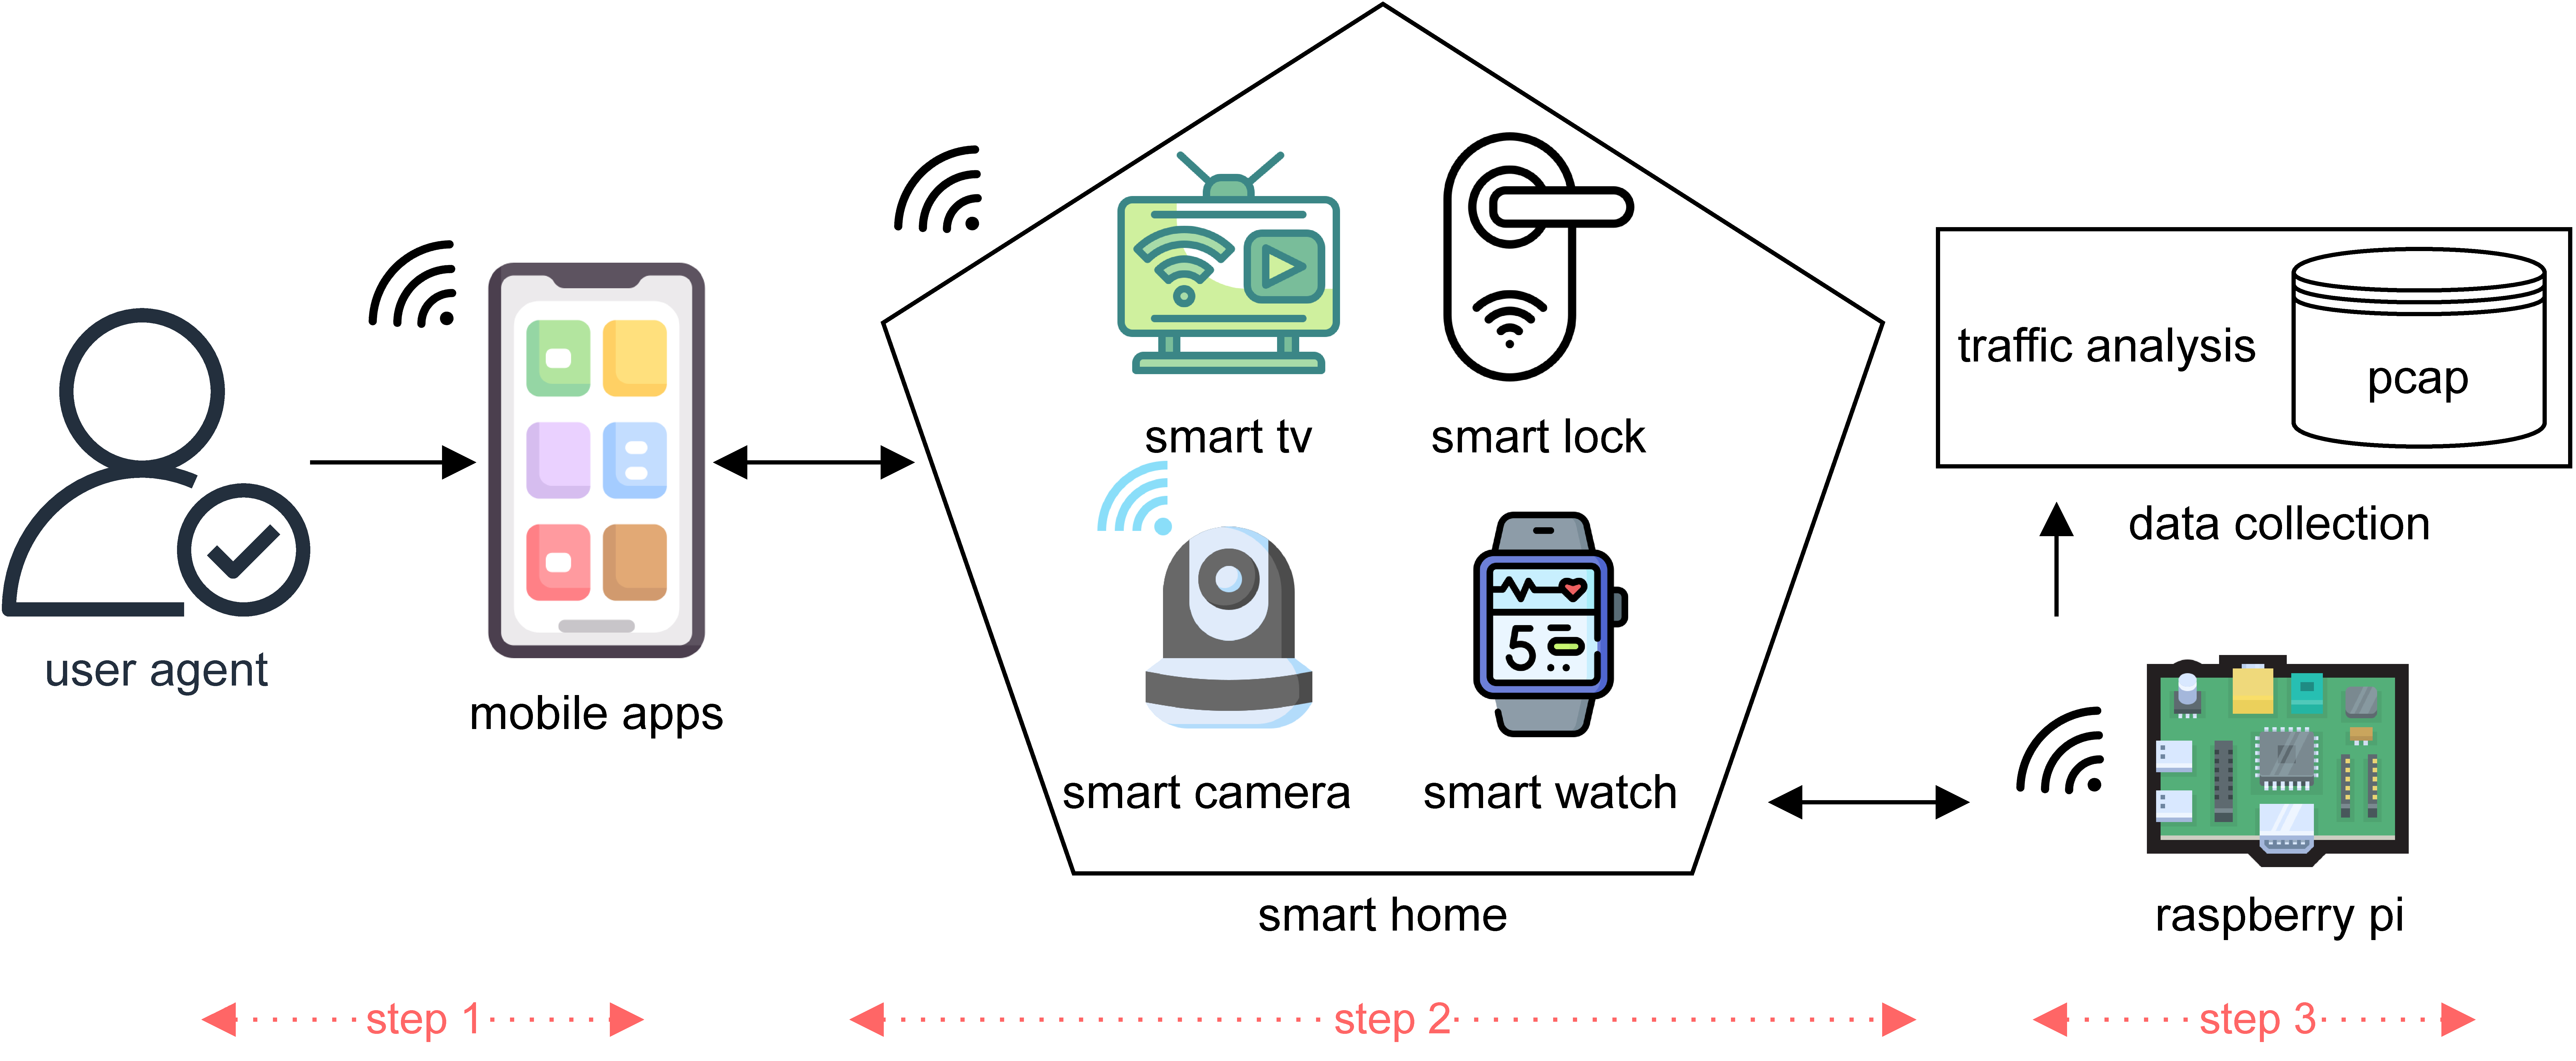
\includegraphics[width=.85\linewidth]{fig/system_setup.pdf}
    \caption{Controlled experiments setup.}
    \Description{Three-step diagram. Step 1: a user agent triggers the update through mobile apps. Step 2: smart home devices, such as a smart TV, smart lock, smart camera, and smart watch, retrieve and install the update over Wi-Fi. Step 3: a Raspberry Pi acting as the wireless access point records the traffic as pcap files for traffic analysis.}
    \label{fig:controlled_sytem_model}
\end{figure}








\subsection{Retrospective Experiments}
In addition to controlled experiments,  we conducted retrospective experiments using previously collected network traffic datasets containing IoT communication traffic.
The dataset used was generated from the Mon(IoT)r Testbed \cite{10.1145/3355369.3355577}, a large-scale IoT experimentation platform. 
The testbed comprises 81 different IoT devices (26 unique models) deployed in the US and the UK, from which 34,586 manually controlled and automated experiments were conducted. 
%The devices span several IoT categories, including cameras, smart hubs, home automation systems, televisions, audio devices, and applications.
To identify the update process characteristics from the retrospective experiments, 
we use update-related keywords, namely  \texttt{software, firmware, update,} and \texttt{download}. 
Matching traffic may signal that an update has been triggered, retrieved, and/or installed on the device. 
%Shorten:
%We selected this dataset because it is not assumed to contain any form of cyberattacks, similar to our controlled dataset, which allows us to investigate network traffic under normal operating conditions.
Based on the update-related traffic observed in the retrospective experiments, we selected the top ten update-related IoT devices for comparison with our controlled experiments.









\subsection{System Model}
We develop a system model for network traffic analysis, similar to the study in \cite{10.1007/978-3-031-30122-3_25},  consisting of three main phases: (i) data preprocessing, (ii)  metadata extraction, and  (iii) parallel execution, as shown in Figure \ref{fig:retrospective_sytem_model}.






In the data preprocessing phase, we use both our dataset from the controlled experiments and the dataset from the retrospective experiments \cite{10.1145/3355369.3355577}.
For the retrospective experiments dataset, we combine it as a whole, without distinguishing between geographic locations or controlled versus uncontrolled experiments, as conducted in the original study \cite{10.1145/3355369.3355577}, this approach is intended to ensure a vendor-agnostic system.
In the metadata extraction phase, we process the packet captures from the dataset, focusing on session-level information relevant to IoT device network traffic.
In the parallel execution phase, metadata extraction is parallelized and deployed on worker nodes, allowing packets to be processed consecutively. 
% shorten
%This parallel pipeline supports efficient network traffic management for object extraction and is designed to be compatible with distributed data processing technologies, such as Apache Hadoop \cite{10.1007/978-3-031-30122-3_25}.
As part of this process, we filter metadata using the aforementioned update-related keywords
%, namely \texttt{software, firmware, update}, and \texttt{download} 
for the retrospective experiments, to extract update-related network traffic.
The final phase of the system model involves distinguishing encrypted from unencrypted network traffic by extracting HTTPS protocol sessions that include the TLS handshake and HTTP protocol sessions, respectively.
This process involves using and modifying the PyShark to disassemble the client and server hello for the TLS handshake, which allows us to reveal, among other things, the entropy, the TLS version, and the cipher suites information.
% the handshake type, 
The results
%of this process 
are stored as extractable metadata in a database, making them ready for further processing in the analysis pipeline, and the encrypted and unencrypted analysis outcomes are retained on the file system.












\begin{figure}[!htbp]
    \centering
    \includegraphics[width=\linewidth]{fig/model.pdf}
    \caption{System model for traffic analysis.}
    \Description{Pipeline diagram. Packet captures from the controlled experiment and from the retrospective experiment, whose metadata is extracted per application, region, and device, flow into a parallel execution environment. There, PyShark worker nodes filter packets with the keywords software, firmware, update, and download, then parse TLS handshakes and extract HTTP objects. Results are written to the file system and as JSON metadata files.}
    \label{fig:retrospective_sytem_model}
\end{figure}




\subsection{Entropy Analysis}
To quantify the uncertainty or randomness in encrypted traffic payloads, we compute three types of entropy: \texttt{Shannon, Rényi}, and \texttt{Tsallis} \cite{6088496},
following the approach in \cite{10.1145/3355369.3355577}. These measures provide different perspectives on the distribution of byte-level frequencies, helping to capture subtle structural differences in encrypted data.

The \texttt{Shannon} entropy is the most widely used measure of information content. For a discrete random variable $X$  with probability distribution ${\{ p_1, p_2, \ldots, p_n \}}$, the Shannon entropy is defined as:
$
    H_{\text{Shannon}}(X) = - \sum_{i=1}^{n} p_i \log_b(p_i)
$,
where $p_i$ is the probability of the $i$-th byte value in the packet payload, and $b$ is the base of the logarithm (in our case, $b=256$ to match the byte range). This entropy quantifies the average uncertainty. %or surprise in observing byte values.
The \texttt{Rényi} entropy is a generalization of Shannon entropy that introduces a tunable parameter $\alpha$ to control the sensitivity to different probability magnitudes:
For order \( \alpha > 0 \) and \( \alpha \ne 1 \):
$
H_{\text{Rényi}}^{(\alpha)}(X) = \frac{1}{1 - \alpha} \log_b \left( \sum_{i=1}^{n} p_i^{\alpha} \right)
$.
When $\alpha \to 1$, Rényi entropy converges to Shannon entropy. Lower values of $\alpha$ emphasize more uniform distributions, while higher values give more weight to dominant probabilities. In our experiments, we use $\alpha = 2$.
The \texttt{Tsallis} entropy is another generalization of Shannon entropy, widely used in non-extensive statistical mechanics. 
In this set-up,
for order \( q > 0 \) and \( q \ne 1 \):
$
H_{\text{Tsallis}}^{(q)}(X) = \frac{1}{q - 1} \left(1 - \sum_{i=1}^{n} p_i^q \right)
$.
Here, $q$ is a real parameter (with $q   \neq 1$), and as $q \to 1$, the formula also reduces to Shannon entropy. Tsallis entropy emphasizes contributions from rare events differently from Rényi entropy, making it useful for capturing tail behavior in the distribution.
In our experiments, we use $q = 1.5$. All three measures are normalized to the $[0,1]$ range for cross-device comparability.








\subsection{Cipher Suites Identification}
\label{subsec:cipher_method}
To analyze the cryptographic mechanisms used during update sessions, we extracted cipher suites information from observed TLS handshakes.
Each cipher suite was represented in its raw 16-bit hexadecimal identifier (as it appears in the handshake).
To enable consistent comparison across devices, versions, and library implementations, these values were then normalized using the IANA TLS cipher suites registry
\cite{IANA_parameters}, which provides a canonical mapping from numeric identifiers to standardized cipher suites names. An example of these names is
\texttt{0xC05C} $\rightarrow$
\path{TLS\_ECDHE\_ECDSA\_WITH\_ARIA\_128\_GCM\_SHA256}.
%Converting cipher suites communication between clients and server from hexadecimal to IANA.



\paragraph{Classification criteria}
Each normalized suite is assigned to one of four categories (insecure, weak, secure, and recommended) based on the community benchmark of \path{ciphersuite.info}, following IETF and NIST guidance \cite{NIST2020-SP800-57}.
The criteria are provided in Table~\ref{tab:cipher_classification}.
\emph{Insecure:} broken suites using obsolete primitives (e.g., NULL, EXPORT, RC4, DES/3DES, anonymous key exchange, or MD5) that should never be used.
\emph{Weak:} deprecated suites relying on outdated primitives, CBC, static RSA, or SHA-1, vulnerable to downgrade, padding-oracle, and retrospective-decryption attacks.
\emph{Secure:} state-of-the-art AEAD-based suites with no known practical attacks, though they may lack forward secrecy.
\emph{Recommended:} TLS~1.3-grade AEAD suites with Perfect Forward Secrecy via ephemeral (EC)DHE, providing the strongest security for modern deployments.

\begin{table}[!htbp]
    \centering
    \caption{Cipher suite classification criteria and  adversarial capability, following the \texttt{ciphersuite.info} benchmark and IETF/NIST~\cite{NIST2020-SP800-57} guidance. AEAD: authenticated encryption with associated data; PFS: (perfect) forward secrecy via ephemeral (EC)DHE.}
    \label{tab:cipher_classification}
    \setlength{\tabcolsep}{3pt}
    \resizebox{\linewidth}{!}{%
    \begin{tabular}{@{} l | >{\raggedright\arraybackslash}p{3.5cm} | >{\raggedright\arraybackslash}p{4.05cm} | >{\raggedright\arraybackslash}p{3.6cm} @{}}
    \toprule
    \textbf{} & \textbf{Defining criteria} & \textbf{Representative suites} & \textbf{Adversarial capability} \\ \hline
    \textbf{Insecure} & Broken primitives: NULL, EXPORT, RC4, DES/3DES, MD5 or anonymous key %exchange 
    & \texttt{RSA\_RC4\_128\_MD5}, \texttt{DH\_anon}, NULL/EXPORT suites & Passive plaintext recovery, MITM/impersonation, key recovery \\ \hline
    \textbf{Weak} & Deprecated primitives: CBC record protection, static RSA (no PFS), or SHA-1 & \texttt{ECDHE\_RSA\_AES\_256\_CBC\_SHA}\newline \texttt{RSA\_AES\_128\_CBC\_SHA} & Padding-oracle (BEAST/Lucky13), downgrade, no-PFS retrospective decryption \\ \hline
    \textbf{Secure} & AEAD with no known practical attack, but may lack PFS & \texttt{ECDHE\_ECDSA\_AES\_128\_CCM}\newline static-RSA AES-GCM suites & Retrospective decryption only if the long-term key later leaks (no PFS) \\ \hline
    \textbf{Recommended} & AEAD \emph{and} PFS; TLS~1.3 -grade (e.g., ECDHE with AES-GCM or ChaCha20) & \texttt{TLS\_AES\_128\_GCM\_SHA256}\newline \texttt{ECDHE\_RSA\_AES\_256\_GCM} & None passively; PFS limits the impact of long-term key compromise \\
    \bottomrule
    \end{tabular}%
    }
\end{table}




%Shorten
%\textbf{Offered vs. negotiated suites.}
%A TLS \texttt{ClientHello} advertises the full list of suites a client is \emph{willing}
%to use, whereas the \texttt{ServerHello} records the single suite actually \emph{negotiated}
%for the session. We analyzed these separately throughout: \texttt{ClientHello} lists are
%treated as capability/offer data that bound a device's downgrade \emph{exposure}, while
%negotiated cipher strength and TLS version are taken from the \texttt{ServerHello}
%(handshake type~2). Conflating the two would overstate weakness, because a client may
%advertise legacy suites that are never selected; keeping them distinct lets us
%distinguish residual capability from realized cryptographic posture.







\subsection{Certificate Security Analysis}
Server authentication in TLS relies on X.509 certificate validation; the entropy and cipher suite analyses that follow characterize how well the channel protects firmware confidentiality once server identity is established.
We performed a multi-stage analysis of X.509 certificates across the selected IoT devices.
First, certificate files were extracted from each device's TLS sessions captured during the controlled experiments.
Second, each X.509 certificate was parsed to extract cryptographic and lifecycle metadata, including public key algorithm, key size, signature algorithm, validity interval (\texttt{notBefore}/\texttt{notAfter}), issuer and subject distinguished names, serial number, and self-signed (SS) status, following X.509 specifications \cite{rfc5280,rfc4055,rfc5480}.
Third, certificates were grouped by NIST SP~800-57 security strength\cite{NIST2020-SP800-57}: 
RSA-1024 maps to up to 80-bit security strength, 
RSA-2048 to 112-bit security strength, and RSA-3072+/EC P-256+ to at least 128-bit security strength. 
Under NIST transition guidance, strengths below 112 bits are disallowed for applying protection, 112 bits is acceptable through 2030 but disallowed for applying protection from 2031 onward (legacy use for processing), and 128 bits and above remain acceptable.
This classification enables a quantitative assessment of whether IoT vendors deploy certificates that meet contemporary cryptographic standards for securing update traffic.
Table~\ref{tab:key_size_consequences} lists the key sizes observed in our captures with their security strength and approval status.

\begin{table}[!htbp]
    \centering
    \caption{Certificate key sizes and corresponding NIST~\cite{NIST2020-SP800-57} security strength.}
    \label{tab:key_size_consequences}
    \setlength{\tabcolsep}{3pt}
    \resizebox{\linewidth}{!}{%
    \begin{tabular}{@{} l | l | l | >{\raggedright\arraybackslash}p{3.3cm} | >{\raggedright\arraybackslash}p{3.4cm} @{}}
    \toprule
    \textbf{Key} & \textbf{Algorithm} & \textbf{Strength} & \textbf{Approval status (SP~800-57, Table~4)} & \textbf{Practical consequence} \\ \hline
    256-bit  & ECC (P-256) & 128 bits       & Acceptable now and beyond 2031 & Small key; fast handshakes; ideal for IoT \\ \hline
    384-bit  & ECC (P-384) & 192 bits       & Acceptable now and beyond 2031 & Higher assurance; slightly slower than P-256 \\ \hline
    1024-bit & RSA         & $\leq 80$ bits & Disallowed for applying protection & Factorable; no protection guarantee \\ \hline
    2048-bit & RSA         & 112 bits       & Acceptable through 2030; disallowed from 2031 & Adequate today; hard expiration date \\ \hline
    4096-bit & RSA         & 128 bits       & Acceptable now and beyond 2031 & Meets target but $16\times$ larger key than ECC-256 \\
    \bottomrule
    \end{tabular}%
    }
\end{table}




\subsection{Vulnerability Analysis}


To investigate the vulnerability implications of  
%insecure and weak 
update-related traffic, we queried the CVE-List \cite{CVE_Program} database using our results derived from insecure and weak cryptographic algorithm implementations. 
To collect and curate the dataset, we followed the methods used in \cite{USMAN2026105019}. 
We search for keyword combinations including \texttt{weak}, \texttt{insecure}, and cipher suite terms.
This allows us to assess the severity of vulnerabilities and identify associated weaknesses of the insecure and weak cipher suites.
%and detail the adversarial capabilities enabled by the software update traffic flows from our cipher suites findings.
To improve traceability, we applied a deterministic mapping workflow: (i) expand each observed insecure/weak suite to canonical IANA names, aliases, and legacy names, (ii) query CVE records using Boolean combinations of protocol family (TLS/SSL), algorithm primitive (e.g., RSA, CBC, RC4, null/anonymous), and weakness terms, (iii) deduplicate by CVE-ID, and (iv) retain only records whose descriptions explicitly reference cryptographic negotiation, certificate validation, or transport-channel confidentiality/integrity weaknesses.

\section{Results}
\label{sec:results}

\subsection{\texorpdfstring{\textcolor{blue}{Update Delivery (RQ1)}}{Update Delivery (RQ1)}}
\label{subsec:profiles}

\paragraph{\textcolor{blue}{How much of the traffic is update traffic}}
\textcolor{blue}{Update flows are a small part of what devices exchange while they update (Table~\ref{tab:funnel}, Figure~\ref{fig:composition}).
In our captures, 715 of 2,219 flows stay on the local network, e.g., tapo-c200's live video to the phone (86\% of its bytes), and most Internet flows serve streaming, telemetry, and time synchronization.
Where an image was transferred, however, the 250 update flows carry almost all bytes: 96 to 100\% for apple-tv, homepod, eufy-cam, xiaomi-cam, reolink-cam, and tapo-c100.
Separating the traffic also corrects individual observations: the only HTTP download of an Apple image in the apple-tv capture is a 5.5\,MB partial fetch of a 2013 restore image for an older Apple~TV model by a system component %(\texttt{TVDisplayAssistant}); 
the update itself arrived over TLS~1.3.}

\begin{figure}[!t]
    \centering
    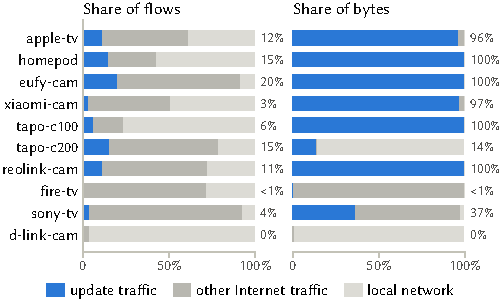
\includegraphics[width=\linewidth]{fig/traffic_composition.pdf}
    \caption{\textcolor{blue}{Share of flows and of bytes that are update traffic, per device, in our captures. Percentages give the update share.}}
    \Description{Two panels of horizontal 100-percent stacked bars, one bar per device. In the share of flows, update traffic is a small part for every device (0 to 20 percent). In the share of bytes, update traffic dominates for apple-tv, homepod, eufy-cam, xiaomi-cam, tapo-c100, and reolink-cam (96 to 100 percent), but not for tapo-c200 (14 percent), fire-tv, sony-tv, and d-link-cam.}
    \label{fig:composition}
\end{figure}

\paragraph{\textcolor{blue}{Delivery paths}}
\textcolor{blue}{Table~\ref{tab:profiles} summarizes how each device received its update, and Figure~\ref{fig:timelines} shows the exchanges of four devices over time.
Six devices fetched their image from vendor or cloud content delivery networks (Apple's own network; Amazon CloudFront and AWS for TP-Link and Eufy; Microsoft Azure and CDN77 for Xiaomi).
For five of them we also observed an update check or a metadata exchange with a separate server, and apple-tv additionally contacted Apple's installation-authorization service (\texttt{gs.apple.com}) before the download.
The update checks and the image transfer need not use the same protection: apple-tv retrieved its catalog and image over TLS~1.3 but most of its metadata and the authorization over TLS~1.2, and tapo-c200 polled TP-Link's device API over TLS for 23~minutes before downloading the image over HTTP.
reolink-cam contacted no update server: its desktop application pushed the image across the local network over a proprietary UDP protocol.}
Of the three devices that were up to date, fire-tv and sony-tv each opened a single update-check connection, and d-link-cam produced no update traffic at all.

\begin{figure*}[!t]
    \centering
    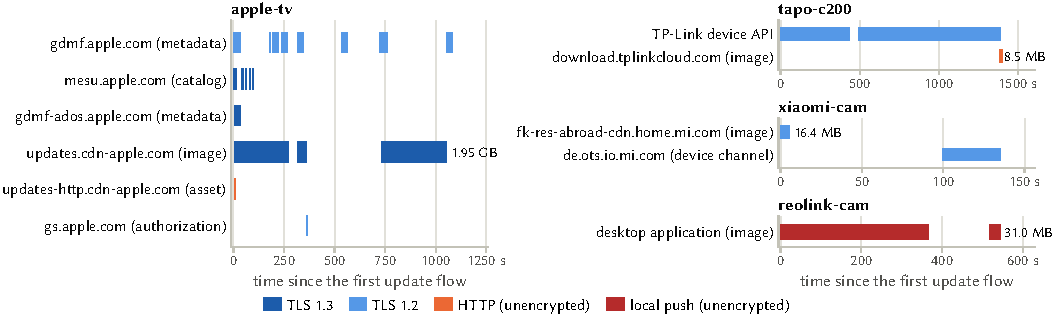
\includegraphics[width=\textwidth]{fig/update_timelines.pdf}
    \caption{\textcolor{blue}{Update exchanges over time for four devices. Each bar is one flow to an update server, from its first to its last packet, colored by how the flow is protected; labels give the size of image transfers. Short flows are widened to stay visible.}}
    \Description{Four timeline panels: apple-tv fills the left half, and tapo-c200, xiaomi-cam, and reolink-cam are stacked on the right. apple-tv: short TLS 1.2 metadata flows to gdmf.apple.com, TLS 1.3 catalog flows to mesu.apple.com, one authorization flow to gs.apple.com, and long TLS 1.3 image flows to updates.cdn-apple.com totalling 1.95 GB over about 1,000 seconds. tapo-c200: many short TLS 1.2 connections to TP-Link's device API for about 450 seconds, a long API connection, and at the end an 8.5 MB HTTP image download. xiaomi-cam: a 16.4 MB TLS 1.2 image download followed by a TLS 1.2 device-channel flow. reolink-cam: two unencrypted local-network flows from the desktop application, 31 MB in total.}
    \label{fig:timelines}
\end{figure*}

\begin{table*}[!t]
    \centering
    \color{blue}
    \caption{How the controlled devices received their updates. 1.2/1.3: TLS version; ECDHE-RSA-GCM: ECDHE key exchange, RSA authentication, AES-GCM (ciphersuite.info: \emph{secure}); TLS~1.3 suites are \emph{recommended}; static-RSA, PSK, and CBC suites are \emph{weak} (Table~\ref{tab:cipher_classes}). n/o: not observed. \textsuperscript{l}Likely update server (multi-purpose device API or unconfirmed check server). \textsuperscript{v}Vendor-published image of the installed firmware line. \textsuperscript{d}Per vendor documentation~\cite{apple-platform-security}.}
    \label{tab:profiles}
    \setlength{\tabcolsep}{2.4pt}
    \footnotesize
    \begin{tabular}{@{} l l l l l l >{\raggedright\arraybackslash}p{2.35cm} @{}}
        \toprule
        \textbf{Device} & \textbf{Firmware} & \textbf{Served from} & \textbf{Check / metadata} & \textbf{Image transfer} & \textbf{Server leaf certificate} & \textbf{Image protection} \\
        \midrule
        apple-tv    & 18.6 $\to$ 26.2       & Apple        & 1.3; 1.2 ECDHE-RSA-GCM                   & 1.3, 1.95\,GB & Apple CA, RSA-2048, 392\,d\textsuperscript{*} & signed, authorized per device\textsuperscript{d} \\
        homepod     & 18.6 $\to$ 26.2       & Apple        & 1.3                                      & 1.3, 1.1\,GB                & hidden by TLS~1.3                  & signed, authorized per device\textsuperscript{d} \\
        eufy-cam    & 2.1.0.2 $\to$ 2.3.1.6 & AWS          & 1.2 ECDHE-RSA-GCM\textsuperscript{l}     & 1.2 ECDHE-RSA-GCM, 19.7\,MB & public CA, RSA-2048, 397\,d        & unknown \\
        xiaomi-cam  & 3.5.1 $\to$ 4.0.9     & Azure, CDN77  & 1.2 PSK-CBC, no cert.\textsuperscript{l} & 1.2 ECDHE-RSA-GCM, 16.4\,MB & public CA, RSA-2048, 385\,d        & unknown \\
        tapo-c100   & 1.0.11 $\to$ 1.4.3    & CloudFront   & n/o                                      & HTTP, 6.7\,MB               & --                                 & signed \\
        tapo-c200   & 1.0.10 $\to$ 1.3.16   & AWS          & 1.2 static RSA-GCM\textsuperscript{l}    & HTTP, 8.5\,MB               & vendor CA, RSA-2048, 15\,y         & signed \\
        reolink-cam & 3.0.0 $\to$ 3.1.0     & desktop app (local) & n/o                                      & proprietary UDP, 31\,MB     & --                                 & no signature found \\
        fire-tv     & up to date            & AWS          & 1.2 ECDHE-RSA-GCM                        & --                          & public CA, RSA-2048, 340\,d        & signed\textsuperscript{v} \\
        sony-tv     & up to date            & AWS          & 1.2 ECDHE-RSA-CBC\textsuperscript{l}     & --                          & public CA, RSA-2048, 393\,d        & unknown \\
        d-link-cam  & up to date            & none observed & --                                       & --                          & --                                 & checksum only (CRC32)\textsuperscript{v} \\
        \bottomrule
        \multicolumn{7}{@{}l}{\textsuperscript{*}TLS~1.2 metadata servers; the TLS~1.3 connections hide the certificate.}
    \end{tabular}
\end{table*}

\paragraph{\textcolor{blue}{2019 baseline}}
\textcolor{blue}{In the retrospective traces, 15 device labels (13 models) contacted 12 confirmed update servers, as shown in Table~\ref{tab:retro}.
Although 97\% of the 2,497 update flows used TLS, four of the 15 labels sent some update traffic over HTTP: Apple~TV fetched signed assets and, once, its update catalog; the Samsung TV fetched firmware headers; the LG TV sent its update check; and the D-Link motion sensor queried its firmware server with its model, firmware version, and MAC address in the URL.}

\begin{table*}[!t]
    \centering
    \color{blue}
    \caption{Confirmed update servers in the 2019 Mon(IoT)r traces. All TLS connections negotiated TLS~1.2; suite abbreviations as in Table~\ref{tab:profiles}. \textsuperscript{a}echodot, t-echodot, echoplus, echospot, firetv, cloudcam. \textsuperscript{b}The thermostat also authenticates with a client certificate valid until 9999.}
    \label{tab:retro}
    \setlength{\tabcolsep}{4pt}
    \footnotesize
    \begin{tabular}{@{} l l l l l @{}}
        \toprule
        \textbf{Update server} & \textbf{Device labels} & \textbf{Protocol} & \textbf{Negotiated suite} & \textbf{Server leaf certificate} \\
        \midrule
        \texttt{softwareupdates.amazon.com} & six Amazon devices\textsuperscript{a} & TLS & ECDHE-RSA-GCM & DigiCert, RSA-2048, 336\,d \\
        \texttt{mesu.apple.com}             & appletv                     & TLS; once HTTP & ECDHE-ECDSA-GCM & Apple, EC P-256, 760\,d \\
        \texttt{gdmf.apple.com}             & appletv                     & TLS            & ECDHE-RSA-GCM   & Apple, RSA-2048, 760\,d \\
        \texttt{updates-http.cdn-apple.com} & appletv                     & HTTP (signed assets) & --        & -- \\
        \texttt{fw-update2.smartthings.com} & smartthings-hub, t-smartthings-hub & TLS     & ECDHE-RSA-GCM   & vendor CA, RSA-1024, 10\,y \\
        \texttt{awsota.linkplay.com}        & allure-speaker              & TLS            & ECDHE-RSA-GCM   & Amazon, RSA-2048, 396\,d \\
        \texttt{hub-updates.winkapp.com}    & wink-hub2                   & TLS            & ECDHE-RSA-GCM   & Comodo, RSA-2048, 730\,d \\
        \texttt{fwuprod.clouddevice.io}     & honeywell-thermostat        & TLS (mutual)   & ECDHE-ECDSA-GCM & vendor CA, EC P-256, 731\,d\textsuperscript{b} \\
        \texttt{otn.samsungcloudcdn.com}    & samsungtv-wired             & HTTP           & --              & -- \\
        \texttt{wrpd.dlink.com}, \texttt{api.dch.dlink.com} & dlink-mov    & HTTP           & --              & -- \\
        \texttt{snu.lge.com}                & lgtv-wired                  & HTTP           & --              & -- \\
        \bottomrule
    \end{tabular}
\end{table*}

\subsection{Channel Protection (RQ2)}
\label{subsec:channel}
Of the seven devices that downloaded an update, four received the image over TLS (apple-tv and homepod over TLS~1.3, eufy-cam and xiaomi-cam over TLS~1.2) and three without encryption.
tapo-c100 and tapo-c200 downloaded their images over HTTP from \texttt{tplinkcloud.com}; the request URLs encode model, hardware revision, and target version, and the images (6.7 and 8.5\,MB) can be recovered byte for byte.
reolink-cam's local push is the only update flow that protocol inspection leaves unclassified.
Its payload has a normalized Shannon entropy of 0.978, 
\textcolor{blue}{which Ren et al.'s ranges would label as likely encrypted, yet it contains UBI, uImage, and SquashFS signatures, and 96\% of sampled 64-byte chunks of the published v3.1 image occur verbatim in the stream: the image travels unencrypted and is merely compressed.
Entropy would thus have misclassified the one flow for which it was needed, so we base encryption status on protocol and content.}

\textcolor{blue}{Figure~\ref{fig:entropy} shows that this is not a corner case.
Per update flow, every TLS connection has a normalized entropy above 0.8, but so do all 14 unencrypted HTTP flows that carry images or signed assets (median 0.99) and the main local push (0.95): a compressed image is as incompressible as ciphertext.
Unencrypted update checks and metadata spread from 0.64 to 0.99 (median 0.73), because some carry binary or encoded content.
An entropy threshold would thus have labelled every unencrypted image transfer in both datasets as encrypted, which is why per-device entropy averages cannot show whether update channels are encrypted.}

\begin{figure}[!t]
    \centering
    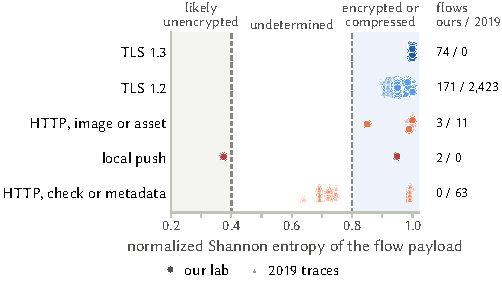
\includegraphics[width=\linewidth]{fig/entropy_by_channel.pdf}
    \caption{\textcolor{blue}{Normalized Shannon entropy of the payload of each update flow (server to device, first 2\,MB), grouped by how protocol inspection classifies the flow; dashed lines are the 0.4 and 0.8 ranges of Ren et al.~\cite{10.1145/3355369.3355577}. Unencrypted image transfers fall in the same range as TLS.}}
    \Description{Strip plot with five rows. TLS 1.3 flows (74, our lab) and TLS 1.2 flows (171 from our lab, 2,423 from 2019) all lie between 0.89 and 1.0. Unencrypted HTTP flows that carry images or assets (3 from our lab, 11 from 2019) lie between 0.85 and 1.0, in the same range. The main local-push flow lies at 0.95 and a small one at 0.37. Unencrypted HTTP update checks and metadata from 2019 (63 flows) lie between 0.64 and 0.99.}
    \label{fig:entropy}
\end{figure}

\paragraph{\textcolor{blue}{What unencrypted requests reveal}}
\textcolor{blue}{Table~\ref{tab:exposure} lists what the unencrypted update requests disclose to a passive observer.
The Tapo image URLs name the camera model, hardware version, region, and the firmware version about to be installed.
In 2019, the LG TV's update check (Base64-encoded, not encrypted) and the D-Link motion sensor's firmware query carried the installed firmware version together with the device's MAC address, a persistent identifier. The Apple~TV named its model, OS version, and build in the User-Agent of its HTTP asset downloads.
This suffices to single out devices that run a vulnerable version.
D-Link's newer upgrade interface, in contrast, encrypts its parameters at the application layer.
TLS hides such fields, but not which update server a device contacts, when, and how much it downloads: we identified every update flow from names sent in cleartext (\S\ref{subsec:attribution}), and a passive observer can do the same.
Nor does an encrypted update channel keep the version secret if other traffic reveals it: apple-tv, whose update traffic is all TLS, sent its model and OS build in the User-Agent of cleartext requests to an Apple identity service.}

\begin{table}[!t]
    \centering
    \color{blue}
    \caption{What unencrypted update requests reveal to a passive observer (values as observed; MAC addresses withheld).}
    \label{tab:exposure}
    \setlength{\tabcolsep}{3pt}
    \footnotesize
    \begin{tabular}{@{} l >{\raggedright\arraybackslash}p{1.55cm} >{\raggedright\arraybackslash}p{4.45cm} @{}}
        \toprule
        \textbf{Device} & \textbf{Request} & \textbf{Revealed} \\
        \midrule
        tapo-c100/c200 & image URL & model and hardware version (C100 v5, C200 v1), region, target version and build \\
        \addlinespace
        \multicolumn{3}{@{}l}{\emph{2019 traces}} \\
        appletv & User-Agent of asset downloads & model (AppleTV5,3), chip, installed OS version and build \\
        lgtv-wired & update check (Base64 XML) & platform, model code, installed firmware version, country, MAC address \\
        dlink-mov & firmware query URL & model (DCH-S150), hardware revision, installed firmware version, MAC address \\
        samsungtv-wired & firmware header URL & firmware line (platform and region), offered version \\
        \bottomrule
    \end{tabular}
\end{table}

\subsection{TLS Settings and Certificates (RQ2)}

\paragraph{Negotiated suites}
\textcolor{blue}{All 2,423 update connections in 2019 negotiated TLS~1.2 with ECDHE and AES-GCM (secure or recommended); no update server selected a weak or insecure suite.
The absence of TLS~1.3 reflects its early adoption after RFC~8446~\cite{rfc8446,holz2020tls13} rather than device limitations.
%: Apple~TV already offered TLS~1.3 suites in 2019, as shown in Figure~\ref{fig:offered}.
In our captures, the Apple devices use TLS~1.3 for catalog and image, and eufy-cam, xiaomi-cam's image server, and fire-tv's update check use ECDHE with AES-GCM.
Three channels negotiate weak suites: tapo-c200's device API selects static RSA (no forward secrecy) in all 144 connections, although the client also offers DHE suites; sony-tv's update check uses an ECDHE-RSA suite in CBC mode; and xiaomi-cam's device channel uses a pre-shared-key CBC suite without any certificate.}

\begin{figure}[!t]
    \centering
    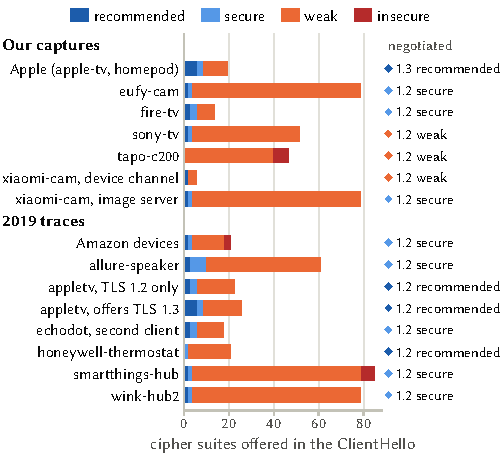
\includegraphics[width=\linewidth]{fig/offered_negotiated.pdf}
    \caption{\textcolor{blue}{Cipher suites offered per client configuration on update channels, by ciphersuite.info category, and the suite negotiated most often (diamond).}}
    \Description{Horizontal stacked bars, one per client configuration, showing how many offered suites fall into each category; most lists are dominated by weak suites, from about 10 to 80 suites long. A column on the right shows the negotiated suite with a colored diamond: TLS 1.3 recommended for Apple, secure or recommended TLS 1.2 suites for most other configurations, and weak suites for sony-tv, tapo-c200, and xiaomi-cam's device channel. tapo-c200, the 2019 Amazon devices, and the 2019 SmartThings hub also offer insecure suites.}
    \label{fig:offered}
\end{figure}

\paragraph{Offered suites}
\textcolor{blue}{Every client configuration offers weak suites, between 55\% (Apple, 11 of 20) and 95\% (eufy-cam and xiaomi-cam, 75 of 79) of its list, which mirrors library defaults rather than negotiated behavior (Figure~\ref{fig:offered}).
Insecure suites are rarer: tapo-c200's device-API client offers RC4 and single-DES suites (7 of 47) and no ECDHE suite at all, and in 2019 the Amazon devices and the SmartThings hub offered RC4.
None of these was ever negotiated, and because the Finished messages protect the offered list (\S\ref{sec:threat}), their presence is a hygiene issue rather than a downgrade path.}

\paragraph{Server certificates}
\textcolor{blue}{Figure~\ref{fig:lifetimes} shows the validity of the leaf certificates that update servers presented.
Leaves from public CAs and from Apple's CA are valid for 340-397 days in our captures and 336-760 days in 2019, within the CA/Browser Forum limits of the time~\cite{cabf-br}, and all use RSA-2048 or EC P-256 (112 or 128~bits).
The exceptions are CAs run by the vendors themselves, which these limits do not bind: TP-Link's device API presents a leaf valid for 15~years, and in 2019 SmartThings' firmware server presented an RSA-1024 leaf (80~bits) valid for ten years, while Honeywell's update server authenticated thermostats by client certificates valid until the year 9999.}

\begin{figure}[!t]
    \centering
    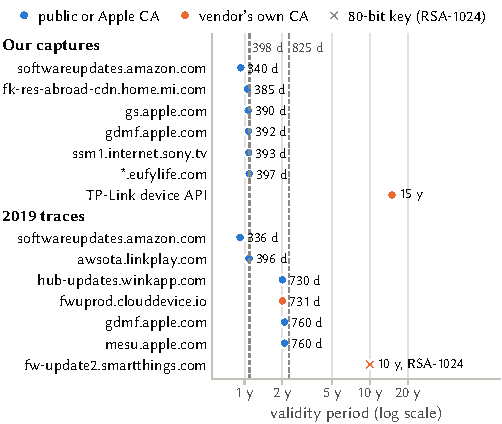
\includegraphics[width=\linewidth]{fig/leaf_lifetimes.pdf}
    \caption{\textcolor{blue}{Validity periods of the leaf certificates presented by update servers (log scale). Dashed lines: CA/Browser Forum limits for publicly trusted certificates (825 days until 2020, 398 days since).}}
    \Description{Dot plot with one row per update server, split into our captures and 2019 traces. Public and Apple certificates cluster between 336 and 760 days, at or below the limits. Two certificates from vendors' own authorities stand out: TP-Link's device API at 15 years, and SmartThings' firmware server in 2019 at 10 years with a 1024-bit RSA key.}
    \label{fig:lifetimes}
\end{figure}

\paragraph{\textcolor{blue}{Revocation}}
\textcolor{blue}{A long-lived certificate is a lasting risk mainly if it cannot be withdrawn after its key is compromised.
Table~\ref{tab:revocation} shows which revocation sources each leaf names, whether the client asks for a stapled OCSP response (visible in TLS~1.3 as well), and whether the device contacted any OCSP or CRL server during the capture.
The Apple devices, fire-tv, and in 2019 the Honeywell thermostat request stapling on every update connection, and where TLS~1.2 makes stapling visible, the server staples a response in 132 of 148 connections.
eufy-cam, xiaomi-cam, sony-tv, and the 2019 Amazon, LinkPlay, and Wink clients neither request stapling nor contact the responder that their public-CA leaf names.
The vendor-CA leaves are the extreme: TP-Link's 15-year leaf names only a revocation list, which tapo-c200 never fetched, and SmartThings' ten-year RSA-1024 leaf names no revocation source at all; the hubs contacted no OCSP or CRL server in 212 captures.}

\begin{table}[!t]
    \centering
    \color{blue}
    \caption{Revocation checking for update-server leaf certificates. \emph{Staple}: the client requests a stapled OCSP response. \emph{Lookup}: the device contacts an OCSP or CRL server during the capture. \textsuperscript{a}From Amazon's own CRL service (18 of 27 captures), not from the issuer of the leaf.}
    \label{tab:revocation}
    \setlength{\tabcolsep}{3pt}
    \footnotesize
    \begin{tabular}{@{} >{\raggedright\arraybackslash}p{2.45cm} l l l l @{}}
        \toprule
        \textbf{Server (clients)} & \textbf{CA, validity} & \textbf{In leaf} & \textbf{Staple} & \textbf{Lookup} \\
        \midrule
        Apple (apple-tv, homepod) & Apple, 390--392\,d & OCSP, CRL & all & apple-tv \\
        Amazon (fire-tv)          & public, 340\,d     & OCSP, CRL & all & no \\
        Eufy, Xiaomi, Sony        & public, 385--397\,d & OCSP, CRL & no & no \\
        TP-Link API (tapo-c200)   & vendor, 15\,y      & CRL       & no  & no \\
        \addlinespace
        \multicolumn{5}{@{}l}{\emph{2019 traces}} \\
        Apple (appletv)           & Apple, 760\,d      & OCSP, CRL & all & 7 of 28 \\
        Honeywell (thermostat)    & vendor, 731\,d     & OCSP, CRL & all & no \\
        Amazon (six devices)      & public, 336\,d     & OCSP, CRL & no  & other\textsuperscript{a} \\
        LinkPlay, Wink            & public, 396/730\,d & OCSP, CRL & no  & no \\
        SmartThings (hub)         & vendor, 10\,y      & none      & no  & no \\
        \bottomrule
    \end{tabular}
\end{table}

\textcolor{blue}{What does this mean for the NIST transition that disallows 112-bit strength for applying protection after 2030~\cite{NIST2020-SP800-57}?
A server's leaf certificate can be replaced on the server at any time, and public-CA leaves are replaced about yearly, so their RSA-2048 keys are not a lasting problem.
A leaf becomes one when it outlives the transition, as TP-Link's does (valid until 2036), or when the device can only trust its vendor's CA: then the trust anchor ships in the firmware, and changing it, or without revocation even withdrawing a compromised key, requires a firmware update, which devices that stop receiving updates before 2031 will not get.}

\subsection{\texorpdfstring{\textcolor{blue}{Image Protection (RQ2)}}{Image Protection (RQ2)}}
\label{subsec:image}
\textcolor{blue}{Figure~\ref{fig:channelimage} combines how each image reached the device with the protection inside it.
The Tapo images, delivered over HTTP, carry a signature block that requires TP-Link's private key, so an on-path adversary can read but not undetectably modify them, provided the device checks the signature.
Apple images are signed and authorized per device at installation time~\cite{apple-platform-security}, and Fire~TV update packages are signed.
The pushed reolink-cam image contains no signature that we could locate, and we could not reproduce its checksum, so this local push is the weakest combination we observed: an unencrypted transfer of an image without evident protection.
The published image of d-link-cam's installed firmware (DCS-5000L v1.05.02) is a uImage protected only by CRC32 header and data checksums; recomputing both after a modification yields an image that passes the format check, so its integrity would rest entirely on the channel.}

\begin{figure}[!t]
    \centering
    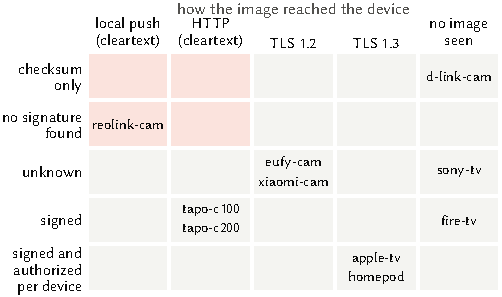
\includegraphics[width=\linewidth]{fig/channel_image.pdf}
    \caption{\textcolor{blue}{How each device's image reached it (columns) versus the protection inside the image (rows). In the shaded cells, an on-path attacker could alter the image without breaking any cryptography, provided the device installs it.}}
    \Description{A grid with five columns (local push unencrypted, HTTP unencrypted, TLS 1.2, TLS 1.3, no image seen) and five rows (checksum only, no signature found, unknown, signed, signed and authorized per device). reolink-cam sits in the shaded cell for a local unencrypted push without a signature; tapo-c100 and tapo-c200 are in HTTP and signed; eufy-cam and xiaomi-cam in TLS 1.2 and unknown; apple-tv and homepod in TLS 1.3 and signed with per-device authorization; d-link-cam, fire-tv, and sony-tv are in the no-image column.}
    \label{fig:channelimage}
\end{figure}

\subsection{\texorpdfstring{\textcolor{blue}{Attack Preconditions (RQ3)}}{Attack Preconditions (RQ3)}}
\label{subsec:preconditions}
\textcolor{blue}{Table~\ref{tab:preconditions} maps each weakness to the attack class it enables.
Only reconnaissance succeeds for a passive adversary without further requirements.
Every tampering path additionally requires that the device installs an image it cannot authenticate, which our data establish at the image level (reolink-cam, d-link-cam) or rule out at that level (Tapo, Apple, Fire~TV), but never at the level of device-side checking.
These are exposure statements: we neither attempted nor observed exploitation on the devices; the only manipulation we performed is the offline D-Link image modification above.}

\begin{table}[!t]
    \centering
    \color{blue}
    \caption{Observed weaknesses, the attacks they enable (CWE~\cite{mitre-cwe}; representative CVE~\cite{CVE_Program}), what the attacks require, and whether our data show the requirement to be met.}
    \label{tab:preconditions}
    \setlength{\tabcolsep}{2pt}
    \footnotesize
    \begin{tabular}{@{} >{\raggedright\arraybackslash}p{2.1cm} >{\raggedright\arraybackslash}p{2.05cm} >{\raggedright\arraybackslash}p{1.8cm} >{\raggedright\arraybackslash}p{2.05cm} @{}}
        \toprule
        \textbf{Weakness (where)} & \textbf{Enables} & \textbf{Requires} & \textbf{Met?} \\
        \midrule
        Unencrypted update check or download (Tapo; 2019: Apple~TV, D-Link, LG, Samsung) & reconnaissance of model and version; tracking by MAC address (CWE-319) & passive on-path $\mathcal{A}$ & yes (Table~\ref{tab:exposure}) \\
        \addlinespace
        Image over HTTP (tapo-c100, tapo-c200) & image substitution (CWE-494) & active $\mathcal{A}$; signature not checked & image signed; checking not observable \\
        \addlinespace
        Unencrypted local push (reolink-cam) & image substitution on the local network (CWE-494) & local access; no image protection & no signature found \\
        \addlinespace
        Checksum-only image (d-link-cam image) & forged image passes check (CWE-345) & unauthenticated delivery channel & no update observed \\
        \addlinespace
        Static RSA key exchange (tapo-c200 API) & decryption of recorded sessions; Bleichenbacher oracle (CWE-327; CVE-2017-13099) & server key compromise or vulnerable server & not observable; leaf valid 15~y \\
        \addlinespace
        CBC suites negotiated (sony-tv, xiaomi-cam) & padding oracle (CWE-327; CVE-2013-0169) & vulnerable implementation; active $\mathcal{A}$ & not observable \\
        \addlinespace
        RC4/DES offered (tapo-c200; 2019: Amazon, SmartThings) & RC4 biases, DES key search (CWE-327; CVE-2013-2566) & server selects them & no; never negotiated \\
        \addlinespace
        RSA-1024 server leaf (2019: SmartThings) & server impersonation (CWE-326) & factoring a 1024-bit key & below NIST minimum \\
        \addlinespace
        Long-lived leaf, revocation never checked (tapo-c200; 2019: SmartThings) & use of a stolen server key until the leaf expires (CWE-299) & key compromise; active $\mathcal{A}$ & not observable; valid 15 and 10~y \\
        \bottomrule
    \end{tabular}
\end{table}

\section{Discussion}
\label{sec:discussion}

\paragraph{\textcolor{blue}{Channel and image together}}
\textcolor{blue}{Channel security alone does not decide update security, but the channel still matters (Figure~\ref{fig:channelimage}).
Apple combines TLS~1.3 with signed images whose installation is authorized per device, the model that SUIT and TUF formalize~\cite{rfc9124,samuel2010tuf}.
TP-Link delivers signed images over HTTP, which exposes model and version but not the image's integrity, while its device API, the likely carrier of update commands, lacks forward secrecy.
Reolink's local push of an image without evident protection, and the checksum-only D-Link image, are the cases in which a network adversary's success would depend on the channel alone.
Most fixes are configuration and signing changes rather than hardware changes: enabling forward-secret key exchange, bounding the lifetime of vendor-issued certificates and checking their revocation, and signing images and update metadata as RFC~9124 prescribes.}

\paragraph{\textcolor{blue}{Measurement choices change the conclusions}}
\textcolor{blue}{Two common shortcuts would have reversed several of our findings.
Keyword matching would have analyzed 6,537 captures, 95\% of which contain no update traffic, and it finds some update servers only by accident (Figure~\ref{fig:keyword}).
Statistics over whole captures would have reported long certificate lifetimes that belong to CAs (up to 50~years), weak certificates that belong to the cameras' local servers (self-signed RSA-1024), weak negotiated suites that belong to local app traffic, and an ``encrypted'' verdict for Reolink's unencrypted image.
Separating update traffic first, by the servers involved, is therefore a prerequisite rather than a refinement.}

\paragraph{\textcolor{blue}{Then and now}}
\textcolor{blue}{The 2019 traces show how the same kinds of devices behaved several years earlier, but the devices in them have since been updated, so we compare practices rather than devices.
Between 2019 and our captures, TLS~1.3 appeared on update channels (Apple), and public-CA certificate lifetimes halved, both following ecosystem-wide changes.
Two practices persisted: update checks and images over HTTP (Samsung, LG, and D-Link in 2019; TP-Link today), and long-lived certificates from vendors' own CAs (SmartThings in 2019; TP-Link today).
Only Apple and Amazon appear in both datasets, and their update channels kept authenticated encryption with forward secrecy throughout.}

\paragraph{Limitations and future work}
\textcolor{blue}{(i)~\emph{Scale}: the controlled set has ten devices, of which seven downloaded an update and three were already up to date, and the 2019 traces contain 15 device labels with update traffic from experiments that were not designed to trigger updates; our results characterize practices, not prevalence.
(ii)~\emph{Identification}: we find update servers through name patterns, large transfers, and manual confirmation, so update commands inside multi-purpose device APIs, which we mark as likely, cannot be separated from other traffic within TLS, and an update served by a server whose name and traffic reveal nothing would be missed.
(iii)~\emph{Passive view}: TLS~1.3 hides certificates; we see neither manifests inside TLS nor whether devices check signatures, validate certificates, or pin their vendor's CA; revocation checks outside a capture would be missed; and the image analysis covers only the images we could obtain.
(iv)~\emph{Exposure, not exploitation}: Table~\ref{tab:preconditions} states what each attack requires; we did not attack the devices.
Future work includes active tests of certificate validation and signature checking on the tested devices, and repeated measurements on more devices with scripted update triggers.}


\section{Conclusion}
\label{sec:conclusion}
We measured how consumer IoT devices receive software updates in our own update experiments and in an earlier public dataset, and separated update traffic from everything else before assessing it.
This separation matters: keyword matching selects protocol vocabulary rather than updates, and statistics over whole captures mix update channels with video streams, local control traffic, and the certificates of unrelated services.
On the update channels themselves, three of the seven devices that downloaded an update received the image unencrypted\textcolor{blue}{, and unencrypted update requests disclose model and firmware version, in 2019 together with MAC addresses}.
Encrypted channels mostly use strong settings, with outdated key exchange and cipher modes as exceptions, and the legacy options that devices offer mirror software defaults rather than what is actually used.
Weak or long-lived server certificates appear only where vendors run their own certificate authorities\textcolor{blue}{, and the devices that trust them never checked whether a certificate had been revoked}.
Whether these weaknesses let an attacker alter an update depends on the signature inside the image, which the two unencrypted downloads carry, and the local push appears to lack, so the channel and the image have to be assessed together.

% ---- Acknowledgments ----
%\begin{credits}
%\subsubsection{\ackname} A bold run-in heading in small font size at the end of the paper is
%used for general acknowledgments, for example: This study was funded
%by X (grant number Y).
%\end{credits}


%Against the 2019 traces this posture has \emph{moved} rather than improved outright: TLS~1.3 now appears where it did not.
%}
%, while the cheapest cameras remain without forward secrecy.
%That the remedies are configuration-level, dropping legacy suite advertisement, shortening certificate lifetimes, and encrypting firmware transfers, makes the gap a matter of vendor practice rather than device capability.}


%An adversary who can observe update traffic can fingerprint devices, extract weak cryptographic parameters, and prioritize targets for further exploitation, a capability that persists even when on-device firmware signature verification is in place.



% Well, i just did the below limitation

%Third, perform controlled, instrumented experiments in laboratory settings.  Run actual update campaigns on instrumented devices to observe the network traffic negotiation outcomes, actual artifact retrievals, signature verification, and certificate-chain validation,  and on-device installation behavior. These experiments will (i) validate entropy-based thresholds, (ii) confirm whether weak cipher offers are actually negotiated in practice, and (iii) enable end-to-end assessment of update integrity and resilience to active attacks.

%\clearpage
%\appendix
%\input{Appendix}




% ---- Acknowledgments ----

%\begin{credits}
%\subsubsection{\ackname} A bold run-in heading in small font size at the end of the paper is
%used for general acknowledgments, for example: This study was funded
%by X (grant number Y).

%\end{credits}



%%
%% Acknowledgments go in the "acks" environment (not a \section); leave it
%% out of the blind submission.
%\begin{acks}
%This study was funded by X (grant number Y).
%\end{acks}

%%
%% Print the bibliography
\printbibliography

%%
%% Appendix
\appendix
\section{Appendix}
%\section{Appendix: Experimental Findings}
\label{app:app}
% SAC 2027: all tables and figures that the text relies on were moved into the
% main body; the appendix keeps only the photo of the test bench.







\begin{figure}[!htbp]
    \centering
    \includegraphics[width=1\linewidth]{fig/devices.jpeg}
    \caption{Controlled experiment devices.}
    \Description{Photograph of the test bench on a desk: an Apple TV, a Fire TV stick with its remote, a HomePod mini, the D-Link, Eufy, Reolink, Tapo C100, Tapo C200, and Xiaomi cameras, and the Raspberry Pi used as the access point, each labelled with its name.}
    \label{fig:devices}
\end{figure}



%% Devices used











%% %% 
%% 





%Abbreviation for update service provider in the above table

%National Institute of Standards and Technology (NIST), University of Colorado (CU), Japan Network Information Center (JNIC),  Vetta Online Ltd (VO),
%FDCservers.net LLC (FDC),
%Aussie Broadband (AB),
%Aliyun Computing Co. Ltd, 
% Chunghwa Telecom Co. Ltd.
%%%%%%%%%
%%%%%%%%


% Update providers

%\textbf{Update supplier:}



%%%%%%%%%
%%%%%%%%









%\textbf{Protocols used:}
%% After removing artifcats and non- related protocols



%%%%%%%
%%%%%%%



























%% Retrospective counterpart of Figure~\ref{fig:entropy_heatmap} (\S\ref{sec:results}).



%% Per-payload entropy distributions, both experiments (moved here from \S\ref{sec:results}).







\begin{comment}
    
\textbf{Security bits distribution:}
Figure~\ref{fig:security_bits_boxplot_all} presents the distribution of security bits across devices with NIST reference thresholds.
The majority of certificates cluster at 112 bits (RSA-2048), with the NIST 128-bit minimum clearly separating strong from transitional deployments.
Tapo-c100 shows the widest spread due to its mix of broken (80-bit) and weak (112-bit) certificates, resulting in the lowest average security strength of 69.3 bits among all devices.
\end{comment}


%% Cipher-suite classification criteria + adversarial capability (addresses formalization request)
%% Cipher-suite classification criteria + adversarial capability (addresses formalization request)












%\textbf{Contacted countries:}










% BLIND REVIEW: the camera frame in these screenshots shows a person; crop or
% blur it before restoring in a blind submission.
% [SAC 2027 page limit] Not cited in the text; excluded so the paper stays within
% the 10-page maximum. Delete this comment/endcomment pair to restore it.
\begin{comment}
\begin{figure}
    \centering
    \begin{subfigure}[b]{0.32\linewidth}
        \centering
        \includegraphics[width=\linewidth]{fig/riolink_uploading.png}
        \caption{Uploading}
        \label{fig:riolink_uploading}
    \end{subfigure}
    \hfill
    \begin{subfigure}[b]{0.32\linewidth}
        \centering
        \includegraphics[width=\linewidth]{fig/riolink_updating.png}
        \caption{Updating}
        \label{fig:riolink_updating}
    \end{subfigure}
    \hfill
    \begin{subfigure}[b]{0.32\linewidth}
        \centering
        \includegraphics[width=\linewidth]{fig/riolink_updated.png}
        \caption{Completed}
        \label{fig:riolink_updated}
    \end{subfigure}
    \caption{Reolink firmware update process.}
    \Description{Three screenshots of the Reolink desktop client: a firmware-update dialog stating that the device is upgrading while the file uploads, the same dialog with the upgrade progress bar, and an update-completed message.}
    \label{fig:riolink_update_process}
\end{figure}
\end{comment}









% [SAC 2027 page limit] Not cited in the text; excluded so the paper stays within
% the 10-page maximum. Delete this comment/endcomment pair to restore it.
\begin{comment}
\begin{figure}[htbp]
    \centering
    \begin{subfigure}[b]{0.48\linewidth}
        \centering
        \includegraphics[width=\linewidth]{fig/apple-tv.jpeg}
        \caption{Update checking}
        \label{fig:apple-tv_checking}
    \end{subfigure}
    \hfill
    \begin{subfigure}[b]{0.48\linewidth}
        \centering
        \includegraphics[width=\linewidth]{fig/apple-tv1.jpeg}
        \caption{Update Downloading}
        \label{fig:apple-tv_downloading}
    \end{subfigure}
    \caption{Apple TV update.}
    \Description{Two photographs of the Apple TV Software Updates screen: a dialog offering the tvOS 26.2 update with download-and-install and later buttons, and a progress bar for the download with about eight minutes remaining.}
    \label{fig:apple_update}
\end{figure}
\end{comment}














%% Certifictate key sizes











%% 






%% %% 
%%  CWE




























































%\begin{figure}
 %   \centering
    %\includegraphics[width=0.9\linewidth]{fig/device_comparison_key_size.pdf}
    %\caption{Per-device comparison of certificate key sizes.}
    %\label{fig:device_comparison_key_size}
%\end{figure}



%\begin{figure}[htbp]
 %   \centering
  %  \includegraphics[width=0.9\linewidth]{fig/device_comparison_strength.pdf}
   % \caption{Per-device certificate strength classification following NIST SP~800-57 guidelines.}
    %\label{fig:device_comparison_strength}
%\end{figure}



%\textbf{Note for now:}
%d-link-cam is already up to date; however, we trigger an update and notice that the device is using  Simple Service Discovery Protocol (SSDP) and provide two info; SEARCH  and SEARCH through *HTTP/1.1.
%Also the sony-tv and fire-tv-stick devices are uptodate.














%\section{Figures from the experiments}















% [SAC 2027 page limit] Not cited in the text; excluded so the paper stays within
% the 10-page maximum. Delete this comment/endcomment pair to restore it.
\begin{comment}
\begin{figure}[htbp]
    \centering

    
    \begin{subfigure}[b]{0.3\linewidth} \centering
        \includegraphics[width=\linewidth]{fig/tapo1_info.png}
        \caption{Information} \label{fig:tapo1_info}
    \end{subfigure}
    \begin{subfigure}[b]{0.3\linewidth} \centering
        \includegraphics[width=\linewidth]{fig/tapo1_updating.png}
        \caption{Updating} \label{fig:tapo_c1_updating}
    \end{subfigure}  
    \begin{subfigure}[b]{0.3\linewidth} \centering
        \includegraphics[width=\linewidth]{fig/tapo1_updated.png}
        \caption{Updated} \label{fig:tapo_c1_updated}
    \end{subfigure}


    
    \caption{Tapo c1 update process}
    \Description{Three smartphone screenshots of the Tapo app for the Tapo C100: the device settings page with the firmware update entry, the new-firmware-available page while updating, and the firmware-up-to-date page showing version 1.4.3.}
    \label{fig:tapo_c1_update}
\end{figure}
\end{comment}



% [SAC 2027 page limit] Not cited in the text; excluded so the paper stays within
% the 10-page maximum. Delete this comment/endcomment pair to restore it.
\begin{comment}
\begin{figure}[htbp]
    \centering

    
    \begin{subfigure}[b]{0.3\linewidth} \centering
        \includegraphics[width=\linewidth]{fig/tapo_info.PNG}
        \caption{tapo information} \label{fig:tapo_c2_info}
    \end{subfigure}
    \begin{subfigure}[b]{0.3\linewidth} \centering
        \includegraphics[width=\linewidth]{fig/tapo_updating.PNG}
        \caption{tapo updating} \label{fig:tapo_c2_updating}
    \end{subfigure}  
    \begin{subfigure}[b]{0.3\linewidth} \centering
        \includegraphics[width=\linewidth]{fig/tapo_updated.PNG}
        \caption{tapo updated} \label{fig:tapo_c2_updated}
    \end{subfigure}


    
    \caption{Tapo C200 update process}
    \Description{Three smartphone screenshots of the Tapo app for the Tapo C200: the device information page listing firmware version 1.0.10, the new-firmware-available page for version 1.3.16 while updating, and the firmware-up-to-date page.}
    \label{fig:tapo_c2_update}
\end{figure}
\end{comment}













% [SAC 2027 page limit] Not cited in the text; excluded so the paper stays within
% the 10-page maximum. Delete this comment/endcomment pair to restore it.
\begin{comment}
\begin{figure}[htbp]
    \centering

    
    \begin{subfigure}[b]{0.3\linewidth} \centering
        \includegraphics[width=\linewidth]{fig/xiaomi_down.PNG}
        \caption{Downloading} \label{fig:xiaomi_downloading}
    \end{subfigure}
    \begin{subfigure}[b]{0.3\linewidth} \centering
        \includegraphics[width=\linewidth]{fig/xiaomi_install.PNG}
        \caption{Updating} \label{fig:xiaomi_updating}
    \end{subfigure}  
    \begin{subfigure}[b]{0.3\linewidth} \centering
        \includegraphics[width=\linewidth]{fig/xiaomi_updated.PNG}
        \caption{Updated} \label{fig:xiaomi_updated}
    \end{subfigure}


    
    \caption{xiaomi   process}
    \Description{Three smartphone screenshots of the Xiaomi camera firmware update: downloading at zero percent with latest version 4.0.9, installing, and updated successfully.}
    \label{fig:update_xiaomi}
\end{figure}
\end{comment}







% [SAC 2027 page limit] Not cited in the text; excluded so the paper stays within
% the 10-page maximum. Delete this comment/endcomment pair to restore it.
\begin{comment}
\begin{figure}[htbp]
    \centering

    
    \begin{subfigure}[b]{0.3\linewidth} \centering
        \includegraphics[width=\linewidth]{fig/eufi_info.PNG}
        \caption{Information} \label{fig:eufy_information}
    \end{subfigure}
    \begin{subfigure}[b]{0.3\linewidth} \centering
        \includegraphics[width=\linewidth]{fig/eufi_downloading.PNG}
        \caption{Updating ($\approx3m$)} \label{fig:eufy_updating}
    \end{subfigure}  
    \begin{subfigure}[b]{0.3\linewidth} \centering
        \includegraphics[width=\linewidth]{fig/eufi_failed.PNG}
        \caption{Failed} \label{fig:eufi_failed}
    \end{subfigure}


    
    \caption{Eufy   process.}
    \Description{Three smartphone screenshots of the Eufy Indoor Cam Pan and Tilt firmware update: update available for version 2.3.1.6, updating at 78 percent with about three minutes left, and an update-failed message with a retry button.}
    \label{fig:update_eufi}
\end{figure}
\end{comment}










%\begin{figure}
 %   \centering
  %  \includegraphics[width=0.9\linewidth]{fig/IMG_8101.png}
   % \caption{Riolink setup}
   % \label{fig:placeholder}
%\end{figure}









% BLIND REVIEW: these screenshots show the Swedish room name "Vardagsrum" and the
% HomePod serial number; crop or blur them before restoring in a blind submission.
% [SAC 2027 page limit] Not cited in the text; excluded so the paper stays within
% the 10-page maximum. Delete this comment/endcomment pair to restore it.
\begin{comment}
\begin{figure}[htbp]
    \centering

    
    \begin{subfigure}[b]{0.3\linewidth} \centering
        \includegraphics[width=\linewidth]{fig/homepod_info.png}
        \caption{Information} \label{fig:homepod_info}
    \end{subfigure}
    \begin{subfigure}[b]{0.3\linewidth} \centering
        \includegraphics[width=\linewidth]{fig/homepod_update.png}
        \caption{Update} \label{fig:homepod_update}
    \end{subfigure}  
    \begin{subfigure}[b]{0.3\linewidth} \centering
        \includegraphics[width=\linewidth]{fig/homepod_updating.png}
        \caption{Updating} \label{fig:omepod_updating}
    \end{subfigure}


    
    \caption{Homepod mini.}
    \Description{Three smartphone screenshots of the Apple Home app for a HomePod mini: the accessory page with an update-available notice, the update details, and the download in progress.}
    \label{fig:homepod_mini}
\end{figure}
\end{comment}







%\begin{figure}[h]
\centering
\scalebox{1}{
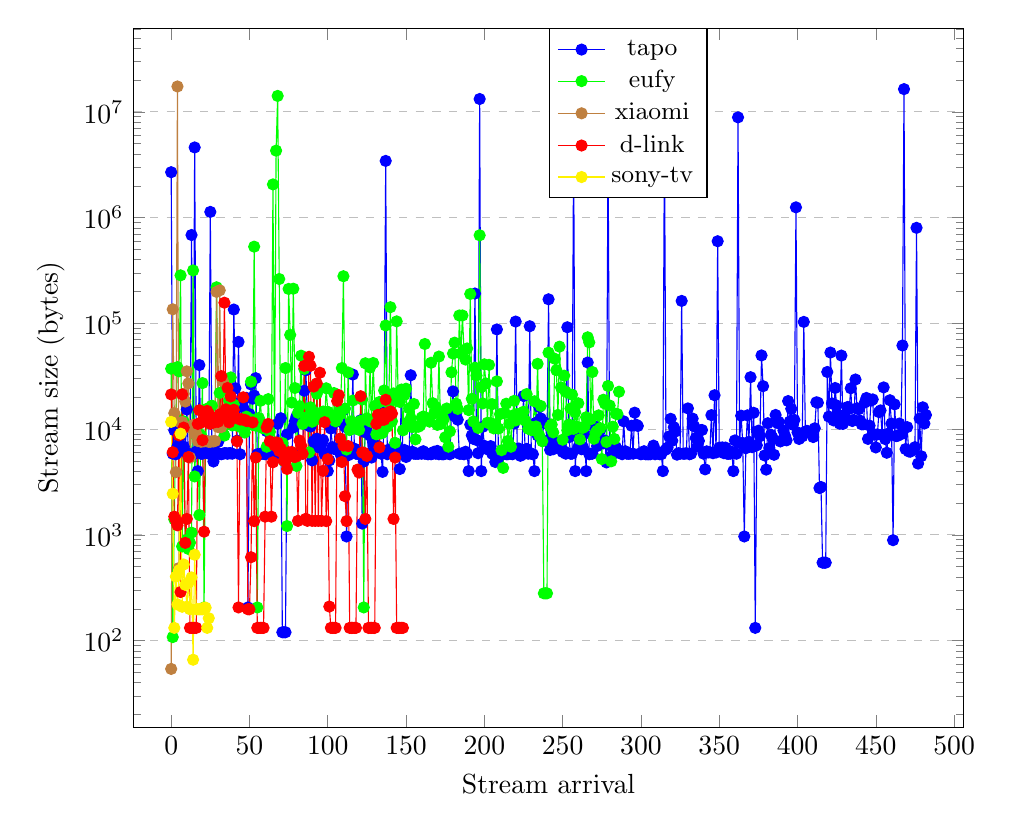
\begin{tikzpicture}[]
\begin{axis}[
%    title={Time (ms)},
    width=\textwidth,           % span entire text width
    %height=0.5\textwidth,       % adjust height as needed
    xlabel={Stream arrival},
    ylabel={ Stream size (bytes)},
    %xmin=0, xmax=11,
    %ymin=0, ymax=60000,
    %xtick={0,1,2,3,4,5,6,7,8,9,10,11},
    %ytick={0, 500,1000,5000,10000,15000,20000,25000,30000,35000,40000,45000,50000,55000,60000},
    legend pos=north west,
    ymajorgrids=true,
	enlarge x limits=0.05,
    grid style=dashed,
    ymode = log,
    %every axis plot/.append style={thick}
    legend style={
        at={(0.5,1)},        % position: (x,y) relative to axis (1,1) is top-right)
        anchor=north west,    % anchor of the legend box
        draw=black,           % optional: add border
        fill=white,           % optional: fill color
        font=\small           % optional: adjust font size
        }
]















 
\addplot[
    color=blue,
    mark=*,
    ]
coordinates {
(0, 2688235)
(1, 5855)
(2, 9757)
(3, 5789)
(4, 6889)
(5, 8522)
(6, 8618)
(7, 6459)
(8, 6841)
(9, 6096)
(10, 15333)
(11, 5789)
(12, 5789)
(13, 684715)
(14, 5789)
(15, 4609320)
(16, 6115)
(17, 4009)
(18, 40348)
(19, 5855)
(20, 5855)
(21, 7327)
(22, 6274)
(23, 6548)
(24, 5855)
(25, 1132768)
(26, 5855)
(27, 4941)
(28, 5996)
(29, 5855)
(30, 7571)
(31, 5855)
(32, 5789)
(33, 5855)
(34, 5921)
(35, 5921)
(36, 5855)
(37, 5921)
(38, 5921)
(39, 5855)
(40, 135183)
(41, 24376)
(42, 7782)
(43, 66810)
(44, 5789)
(45, 19034)
(46, 16080)
(47, 11280)
(48, 19752)
(49, 206)
(50, 13861)
(51, 26417)
(52, 19391)
(53, 20753)
(54, 30333)
(55, 5789)
(56, 5789)
(57, 5855)
(58, 5855)
(59, 5855)
(60, 5789)
(61, 9564)
(62, 6058)
(63, 5789)
(64, 5855)
(65, 5855)
(66, 5855)
(67, 5855)
(68, 11212)
(69, 5855)
(70, 12679)
(71, 120)
(72, 120)
(73, 120)
(74, 8903)
(75, 5921)
(76, 5855)
(77, 5789)
(78, 10353)
(79, 11865)
(80, 13215)
(81, 12325)
(82, 5855)
(83, 5921)
(84, 5855)
(85, 23058)
(86, 36058)
(87, 12498)
(88, 10736)
(89, 10578)
(90, 5057)
(91, 7685)
(92, 7021)
(93, 8126)
(94, 6723)
(95, 6709)
(96, 7237)
(97, 7886)
(98, 5789)
(99, 5855)
(100, 4009)
(101, 5057)
(102, 10121)
(103, 6757)
(104, 6490)
(105, 11640)
(106, 6473)
(107, 6671)
(108, 5855)
(109, 5855)
(110, 15168)
(111, 10536)
(112, 966)
(113, 5651)
(114, 6820)
(115, 6118)
(116, 32815)
(117, 6537)
(118, 5855)
(119, 5855)
(120, 5789)
(121, 12129)
(122, 1278)
(123, 4941)
(124, 9324)
(125, 10563)
(126, 5789)
(127, 8687)
(128, 5381)
(129, 7496)
(130, 6459)
(131, 6709)
(132, 6907)
(133, 6544)
(134, 5855)
(135, 3943)
(136, 14394)
(137, 3438605)
(138, 5789)
(139, 6404)
(140, 6114)
(141, 5855)
(142, 5789)
(143, 6217)
(144, 7030)
(145, 5789)
(146, 4195)
(147, 23251)
(148, 5855)
(149, 6349)
(150, 5451)
(151, 5789)
(152, 5789)
(153, 32312)
(154, 6114)
(155, 5855)
(156, 5855)
(157, 5855)
(158, 5855)
(159, 5921)
(160, 5855)
(161, 6181)
(162, 5855)
(163, 5855)
(164, 5789)
(165, 5855)
(166, 5789)
(167, 5855)
(168, 6115)
(169, 5855)
(170, 6223)
(171, 5789)
(172, 5855)
(173, 5789)
(174, 5789)
(175, 5855)
(176, 6180)
(177, 5855)
(178, 5789)
(179, 14163)
(180, 22737)
(181, 13268)
(182, 14144)
(183, 12270)
(184, 5855)
(185, 5855)
(186, 5855)
(187, 5789)
(188, 6114)
(189, 5855)
(190, 4009)
(191, 11028)
(192, 8741)
(193, 8094)
(194, 191473)
(195, 7886)
(196, 5921)
(197, 13230348)
(198, 4009)
(199, 10518)
(200, 6955)
(201, 6556)
(202, 6459)
(203, 6655)
(204, 6907)
(205, 5855)
(206, 5789)
(207, 4888)
(208, 87641)
(209, 5346)
(210, 5789)
(211, 5789)
(212, 6245)
(213, 5855)
(214, 5789)
(215, 5789)
(216, 5921)
(217, 5855)
(218, 5789)
(219, 11284)
(220, 104014)
(221, 6490)
(222, 6555)
(223, 5592)
(224, 5724)
(225, 20555)
(226, 6301)
(227, 6505)
(228, 5855)
(229, 93945)
(230, 5855)
(231, 5789)
(232, 4009)
(233, 11489)
(234, 8735)
(235, 16191)
(236, 12639)
(237, 7871)
(238, 11667)
(239, 11329)
(240, 7673)
(241, 168914)
(242, 6353)
(243, 8258)
(244, 6459)
(245, 6841)
(246, 7171)
(247, 7236)
(248, 7525)
(249, 7222)
(250, 6088)
(251, 6172)
(252, 5855)
(253, 91875)
(254, 8382)
(255, 5855)
(256, 5855)
(257, 4903915)
(258, 4009)
(259, 8552)
(260, 6757)
(261, 8258)
(262, 6459)
(263, 6709)
(264, 9027)
(265, 4009)
(266, 42637)
(267, 5789)
(268, 5855)
(269, 5855)
(270, 10707)
(271, 8164)
(272, 6913)
(273, 9516)
(274, 9812)
(275, 7794)
(276, 7328)
(277, 7805)
(278, 4840)
(279, 5028493)
(280, 5373)
(281, 6933)
(282, 5856)
(283, 5922)
(284, 6752)
(285, 6030)
(286, 6024)
(287, 6184)
(288, 5789)
(289, 11849)
(290, 6181)
(291, 5855)
(292, 5855)
(293, 5855)
(294, 10758)
(295, 5855)
(296, 14309)
(297, 11010)
(298, 10710)
(299, 5855)
(300, 5789)
(301, 5855)
(302, 6182)
(303, 5789)
(304, 5789)
(305, 5789)
(306, 5789)
(307, 5921)
(308, 6987)
(309, 5789)
(310, 6182)
(311, 5855)
(312, 5789)
(313, 5789)
(314, 4009)
(315, 6645833)
(316, 6410)
(317, 6685)
(318, 8535)
(319, 12515)
(320, 7761)
(321, 10440)
(322, 9493)
(323, 5736)
(324, 5922)
(325, 5855)
(326, 163083)
(327, 5855)
(328, 5855)
(329, 5921)
(330, 15703)
(331, 5789)
(332, 5855)
(333, 12582)
(334, 10635)
(335, 8244)
(336, 6848)
(337, 7741)
(338, 9754)
(339, 9812)
(340, 5855)
(341, 4165)
(342, 6164)
(343, 6023)
(344, 6045)
(345, 13561)
(346, 5921)
(347, 20918)
(348, 6011)
(349, 598002)
(350, 6676)
(351, 6657)
(352, 6709)
(353, 5922)
(354, 6686)
(355, 5855)
(356, 5855)
(357, 5855)
(358, 6116)
(359, 4009)
(360, 7820)
(361, 5855)
(362, 8873587)
(363, 7404)
(364, 13393)
(365, 7398)
(366, 966)
(367, 6595)
(368, 13499)
(369, 7581)
(370, 30985)
(371, 6752)
(372, 14269)
(373, 132)
(374, 7027)
(375, 9659)
(376, 8557)
(377, 49767)
(378, 25477)
(379, 5640)
(380, 4142)
(381, 11370)
(382, 6625)
(383, 8854)
(384, 8298)
(385, 5719)
(386, 13615)
(387, 11458)
(388, 11697)
(389, 7647)
(390, 7813)
(391, 9710)
(392, 8681)
(393, 7835)
(394, 18425)
(395, 11750)
(396, 15583)
(397, 10999)
(398, 12219)
(399, 1250593)
(400, 9315)
(401, 8073)
(402, 8814)
(403, 8537)
(404, 103260)
(405, 9433)
(406, 9628)
(407, 9502)
(408, 9437)
(409, 9484)
(410, 8412)
(411, 10184)
(412, 17927)
(413, 17783)
(414, 2771)
(415, 2837)
(416, 546)
(417, 546)
(418, 546)
(419, 34702)
(420, 13137)
(421, 52973)
(422, 17517)
(423, 12090)
(424, 24498)
(425, 16731)
(426, 13630)
(427, 11247)
(428, 49601)
(429, 11196)
(430, 13528)
(431, 12342)
(432, 16198)
(433, 15585)
(434, 24341)
(435, 11936)
(436, 12196)
(437, 29472)
(438, 15748)
(439, 15419)
(440, 12020)
(441, 11102)
(442, 11115)
(443, 17876)
(444, 19718)
(445, 8080)
(446, 10801)
(447, 18646)
(448, 19106)
(449, 8915)
(450, 6709)
(451, 8913)
(452, 14483)
(453, 15035)
(454, 8872)
(455, 24809)
(456, 8044)
(457, 5978)
(458, 9083)
(459, 18767)
(460, 11287)
(461, 891)
(462, 17138)
(463, 8588)
(464, 8658)
(465, 11287)
(466, 8939)
(467, 61790)
(468, 16411474)
(469, 6479)
(470, 10446)
(471, 6155)
(472, 6118)
(473, 6342)
(474, 6413)
(475, 6752)
(476, 800763)
(477, 4721)
(478, 12618)
(479, 5544)
(480, 16077)
(481, 11289)
(482, 13598)

  
};





\addplot[
    color=green,
    mark=*,
    ]
    coordinates {
(0, 37247)
(1, 108)
(2, 1401)
(3, 12793)
(4, 38590)
(5, 35193)
(6, 284491)
(7, 778)
(8, 11835)
(9, 778)
(10, 898)
(11, 736)
(12, 844)
(13, 1050)
(14, 316719)
(15, 3570)
(16, 8719)
(17, 8601)
(18, 1540)
(19, 8772)
(20, 27253)
(21, 206)
(22, 7777)
(23, 15608)
(24, 14285)
(25, 11834)
(26, 16666)
(27, 11437)
(28, 12595)
(29, 219418)
(30, 11552)
(31, 22013)
(32, 10736)
(33, 10228)
(34, 8688)
(35, 24216)
(36, 12823)
(37, 18598)
(38, 30844)
(39, 10834)
(40, 17101)
(41, 12453)
(42, 12165)
(43, 10654)
(44, 11856)
(45, 10694)
(46, 11455)
(47, 9280)
(48, 13126)
(49, 12513)
(50, 12535)
(51, 28121)
(52, 10948)
(53, 531537)
(54, 10775)
(55, 206)
(56, 12748)
(57, 18529)
(58, 10264)
(59, 11138)
(60, 10078)
(61, 6816)
(62, 19221)
(63, 9441)
(64, 7510)
(65, 2061571)
(66, 7473)
(67, 4298447)
(68, 14153432)
(69, 262713)
(70, 7356)
(71, 7393)
(72, 5002)
(73, 37801)
(74, 1212)
(75, 211669)
(76, 77788)
(77, 17854)
(78, 212714)
(79, 24487)
(80, 4484)
(81, 14274)
(82, 16491)
(83, 49517)
(84, 11209)
(85, 37047)
(86, 12267)
(87, 13052)
(88, 6023)
(89, 16086)
(90, 11742)
(91, 14558)
(92, 26069)
(93, 21604)
(94, 12576)
(95, 12498)
(96, 12524)
(97, 14662)
(98, 12624)
(99, 24324)
(100, 14593)
(101, 13123)
(102, 12613)
(103, 13358)
(104, 21937)
(105, 11848)
(106, 12597)
(107, 14705)
(108, 13809)
(109, 37802)
(110, 279096)
(111, 15618)
(112, 6409)
(113, 34372)
(114, 9792)
(115, 11847)
(116, 18636)
(117, 10485)
(118, 10122)
(119, 10545)
(120, 9850)
(121, 11964)
(122, 19047)
(123, 206)
(124, 41940)
(125, 12643)
(126, 12086)
(127, 38274)
(128, 11690)
(129, 42212)
(130, 16570)
(131, 8928)
(132, 9509)
(133, 18059)
(134, 9101)
(135, 9248)
(136, 23208)
(137, 95506)
(138, 10543)
(139, 17634)
(140, 142263)
(141, 11867)
(142, 21768)
(143, 7426)
(144, 104481)
(145, 18409)
(146, 18079)
(147, 23667)
(148, 9734)
(149, 21080)
(150, 24102)
(151, 11540)
(152, 15708)
(153, 12654)
(154, 10435)
(155, 17293)
(156, 8001)
(157, 10560)
(158, 10551)
(159, 10847)
(160, 12839)
(161, 13169)
(162, 63838)
(163, 12526)
(164, 12541)
(165, 11765)
(166, 42435)
(167, 17607)
(168, 14105)
(169, 16224)
(170, 10962)
(171, 48557)
(172, 11166)
(173, 13370)
(174, 12374)
(175, 8366)
(176, 15682)
(177, 6821)
(178, 9529)
(179, 34455)
(180, 51853)
(181, 65736)
(182, 17386)
(183, 15532)
(184, 118747)
(185, 51926)
(186, 118779)
(187, 55682)
(188, 45481)
(189, 57941)
(190, 15124)
(191, 189675)
(192, 19339)
(193, 11801)
(194, 38158)
(195, 32099)
(196, 10260)
(197, 680699)
(198, 24974)
(199, 17504)
(200, 40986)
(201, 27038)
(202, 11489)
(203, 40501)
(204, 11406)
(205, 17217)
(206, 10162)
(207, 11054)
(208, 28283)
(209, 10127)
(210, 13844)
(211, 6322)
(212, 4298)
(213, 14238)
(214, 17399)
(215, 7733)
(216, 11219)
(217, 6809)
(218, 13434)
(219, 18502)
(220, 12076)
(221, 13900)
(222, 13347)
(223, 13898)
(224, 14100)
(225, 14602)
(226, 12038)
(227, 21440)
(228, 10103)
(229, 10662)
(230, 9796)
(231, 9850)
(232, 18333)
(233, 10592)
(234, 41437)
(235, 8753)
(236, 16571)
(237, 7679)
(238, 280)
(239, 280)
(240, 280)
(241, 52837)
(242, 10535)
(243, 11046)
(244, 9315)
(245, 46259)
(246, 36103)
(247, 13625)
(248, 60256)
(249, 24738)
(250, 7941)
(251, 32007)
(252, 22526)
(253, 9766)
(254, 11035)
(255, 15657)
(256, 21173)
(257, 10060)
(258, 14468)
(259, 10565)
(260, 17549)
(261, 8002)
(262, 10320)
(263, 10299)
(264, 10619)
(265, 12950)
(266, 73855)
(267, 66101)
(268, 12397)
(269, 34691)
(270, 8102)
(271, 9207)
(272, 9651)
(273, 13502)
(274, 10221)
(275, 5215)
(276, 18963)
(277, 17452)
(278, 7556)
(279, 25581)
(280, 16729)
(281, 4958)
(282, 10537)
(283, 8074)
(284, 13977)
(285, 13876)
(286, 22563)
};

    




\addplot[
    color=brown,
    mark=*,
    ]
    coordinates {
(0, 54)
(1, 135792)
(2, 14164)
(3, 3921)
(4, 17385382)
(5, 486)
(6, 11550)
(7, 11634)
(8, 21571)
(9, 18228)
(10, 35166)
(11, 27089)
(12, 5392)
(13, 10187)
(14, 10954)
(15, 9041)
(16, 9041)
(17, 7720)
(18, 7720)
(19, 7600)
(20, 7666)
(21, 7666)
(22, 7720)
(23, 7666)
(24, 7600)
(25, 7600)
(26, 7666)
(27, 7654)
(28, 7720)
(29, 198616)
(30, 10447)
(31, 205314)
(32, 10447)
(33, 28504)
};













\addplot[
    color=red,
    mark=*,
    ]
    coordinates {
(0, 21277)
(1, 6045)
(2, 1487)
(3, 1363)
(4, 1231)
(5, 8720)
(6, 288)
(7, 21288)
(8, 10336)
(9, 840)
(10, 1415)
(11, 5438)
(12, 132)
(13, 132)
(14, 132)
(15, 132)
(16, 132)
(17, 11203)
(18, 15088)
(19, 11501)
(20, 7866)
(21, 1072)
(22, 13603)
(23, 14868)
(24, 14011)
(25, 11218)
(26, 12220)
(27, 12685)
(28, 11656)
(29, 12393)
(30, 11733)
(31, 13793)
(32, 31720)
(33, 13296)
(34, 156861)
(35, 15379)
(36, 24494)
(37, 11570)
(38, 20385)
(39, 14452)
(40, 15246)
(41, 12856)
(42, 7675)
(43, 206)
(44, 12328)
(45, 12408)
(46, 19990)
(47, 12238)
(48, 11929)
(49, 198)
(50, 198)
(51, 615)
(52, 11572)
(53, 1349)
(54, 5384)
(55, 132)
(56, 132)
(57, 132)
(58, 132)
(59, 132)
(60, 1487)
(61, 10368)
(62, 11206)
(63, 7681)
(64, 1487)
(65, 4859)
(66, 7023)
(67, 7485)
(68, 7417)
(69, 6215)
(70, 6544)
(71, 6085)
(72, 5045)
(73, 4912)
(74, 4199)
(75, 6042)
(76, 5727)
(77, 6078)
(78, 5512)
(79, 5450)
(80, 5534)
(81, 1357)
(82, 7790)
(83, 6982)
(84, 5848)
(85, 39652)
(86, 1420)
(87, 1357)
(88, 48281)
(89, 39724)
(90, 1357)
(91, 25247)
(92, 1357)
(93, 27079)
(94, 1357)
(95, 34122)
(96, 1357)
(97, 4032)
(98, 11618)
(99, 1349)
(100, 5198)
(101, 210)
(102, 132)
(103, 132)
(104, 132)
(105, 132)
(106, 18444)
(107, 20975)
(108, 8152)
(109, 4886)
(110, 6994)
(111, 2322)
(112, 1349)
(113, 6910)
(114, 132)
(115, 132)
(116, 132)
(117, 132)
(118, 132)
(119, 4138)
(120, 3886)
(121, 20468)
(122, 6005)
(123, 5991)
(124, 1415)
(125, 5576)
(126, 132)
(127, 132)
(128, 132)
(129, 132)
(130, 132)
(131, 11213)
(132, 13646)
(133, 6718)
(134, 12170)
(135, 13905)
(136, 12264)
(137, 18954)
(138, 14166)
(139, 13290)
(140, 14726)
(141, 14023)
(142, 1415)
(143, 5384)
(144, 132)
(145, 132)
(146, 132)
(147, 132)
(148, 132)
};




















\addplot[
    color=yellow,
    mark=*,
    ]
    coordinates {
(0, 11705)
(1, 2449)
(2, 132)
(3, 403)
(4, 220)
(5, 462)
(6, 9060)
(7, 209)
(8, 525)
(9, 337)
(10, 209)
(11, 353)
(12, 198)
(13, 396)
(14, 66)
(15, 648)
(16, 198)
(17, 198)
(18, 198)
(19, 198)
(20, 198)
(21, 205)
(22, 205)
(23, 132)
(24, 163)
};











\legend{tapo, eufy, xiaomi, d-link, sony-tv}
\end{axis}
\end{tikzpicture}
}
 \caption[justification=centering]{Stream size.}
  \label{fig:stream_size}
\end{figure}


\begin{comment}
    

\section{Entropy}

Figure \ref{fig:device_comparison} contains six time-series subplots (a-f), each showing entropy measures computed for a sequence of update-related network sessions from a single device/platform. The x-axis in every subplot is the session index (consecutive update-related sessions captured for that device); the x-axis length differs per device because the number of sessions varies. 
The y-axis is normalized entropy (range 0.00-1.00). 
Each plot overlays three entropy metrics: Shannon (blue), Rényi (red), and Tsallis (yellow). 
The legend in each subplot identifies these three traces.
To describe these panel-by-panel observations:
\begin{itemize}
    \item [\textbullet]
    (a) appletv: Shannon and Rényi entropies sit roughly in the 0.65-0.85 band and show gentle, correlated oscillations across sessions; Rényi is consistently slightly lower than Shannon. 
    Tsallis is much higher ($\approx$0.90-0.99) and relatively flat, indicating a systematic offset between Tsallis and the other two metrics for this device.

    \item [\textbullet]
    (b) roku-tv: Entropy traces show larger short-term variability, especially at small session indices where all three metrics fluctuate sharply. After the initial volatility, Shannon and Rényi settle into a band around 0.50-0.70, while Tsallis remains high but exhibits larger swings than in (a), briefly approaching 1.0 at several points.

    \item [\textbullet]
    (c) fire-tv: All three metrics are relatively stable with Shannon and Rényi around 0.65-0.80 and Tsallis near 0.95-1.00. The traces are closely correlated, with modest session-to-session variation and no large outliers.
    
    \item [\textbullet]
    (d) samsung-tv: Shannon and Rényi gradually trend toward slightly lower values ($\approx$0.60-0.75) with a few small spikes; Tsallis again remains near the top of the scale ($\approx$0.93-0.99). A localized increase appears in the later sessions.

    \item [\textbullet]
    (e) echo-dot: Shannon and Rényi typically lie in the 0.55-0.75 range; Rényi shows more pronounced short dips than Shannon. Tsallis is near 0.95 for most of the sequence but drops sharply near the very end (a clear deviation from the earlier pattern).

    \item [\textbullet]
    (f) echo-plus: Shannon is fairly stable around 0.70-0.80. Rényi displays the greatest volatility among all devices, with multiple low spikes (down toward 0.30-0.40) interspersed with higher values. 
    Tsallis remains high and steady ($\approx$0.90-0.98).

\end{itemize}

To summarize,
the three entropy measures produce distinct numerical ranges for the same sessions: Tsallis consistently returns the highest values, Shannon intermediate, and Rényi the lowest (and most volatile in some cases). 
This is expected because these metrics emphasize distributional features differently; the visual separation highlights the value of comparing multiple entropy formulations rather than relying on a single entropy measure.






For the analyzed IoT device, each device exhibits a characteristic entropy profile (level, volatility, and occasional abrupt changes). 
Such profiles can be used to (a) flag anomalous sessions, (b) distinguish device families,  or (c) infer when a session is highly encrypted versus plaintext (e.g., sustained high entropy is consistent with encrypted/pseudo-random payloads).
On the anomalies and session-level diagnostics. 
Sharp drops or spikes - for example, the end-of-sequence drop in Tsallis for echodot, or the low Rényi spikes in echoplus - merit inspection: they may indicate transitions between encrypted and plaintext transfers, short control packets, or extraction artifacts.










Table ?? presents the entropy analysis results for update-related sessions across six IoT devices.  
The reported values represent the average of session-level entropy measures, aggregated per device,
providing complementary perspectives on the randomness and potential encryption of the payload data.
Across all devices, Tsallis entropy values are consistently the highest.
This suggests that Tsallis entropy is more sensitive in detecting high-randomness distributions in the payload, making it an effective indicator of encrypted traffic. Shannon entropy results show moderate-to-high values, with apple-tv and  fire-tv   exhibiting the strongest indications of encrypted traffic. 
Rényi entropy values are consistently lower than both Shannon and Tsallis, which may reflect its sensitivity to dominant probability distributions in the data.

%In terms of device-specific trends, Fire TV and Apple TV show the strongest alignment across all three entropy metrics, supporting the inference that these devices handle a greater proportion of encrypted update-related traffic. Roku TV consistently reports the lowest values across the three metrics, indicating that its update-related sessions may include a higher proportion of unencrypted or weakly encrypted traffic. Samsung TV, Echo Dot, and Echo Plus fall between these two extremes, showing moderate entropy values but with Tsallis approaching near-maximum for all.




\end{comment}

    






\begin{comment}
    












%%%%%%%%%%%%%%%%%55
%%%%%%%%%%%%%%%%5


\begin{figure*}[htb]
    \centering
    % --- First row: 2 figures ---
    \begin{subfigure}{0.48\textwidth}
        \centering
        \includegraphics[width=\linewidth]{fig/tapo_entropy_plot.pdf}
        \caption{Tapo entropy}
    \end{subfigure}
    %\hfill
    \begin{subfigure}{0.48\textwidth}
        \centering
        \includegraphics[width=\linewidth]{fig/dlink_entropy_plot.pdf}
        \caption{Dlink entropy}
    \end{subfigure}

    % --- Second row: 3 figures ---
    \begin{subfigure}{0.48\textwidth}
        \centering
        \includegraphics[width=\linewidth]{fig/eufy_entropy_plot.pdf}
        \caption{Eufy entropy}
    \end{subfigure}
    %\hfill
    \begin{subfigure}{0.48\textwidth}
        \centering
        \includegraphics[width=\linewidth]{fig/xiaomi_entropy_plot.pdf}
        \caption{Xiaomi entropy}
    \end{subfigure}
   % \hfill
   % \begin{subfigure}{0.32\textwidth}
    %    \centering
     %   \includegraphics[width=\linewidth]{fig/sony_entropy_plot.pdf}
      %  \caption{Sony-tv entropy}
    %\end{subfigure}

    \caption{Entropy plots for controlled experiments.}
    \label{fig:five-entropy}
\end{figure*}






\end{comment}


\begin{comment}
    
%%%%%%%%%%%%%%%%%%%%%%%
%%%%%%%%%%%%%%

\begin{figure}
    \centering
    % First row
    \begin{subfigure}[b]{0.48\textwidth}
        \centering
        \includegraphics[width=\textwidth]{fig/appletv.pdf}
        \caption{appletv}
        \label{fig:appletv}
    \end{subfigure}
    \begin{subfigure}[b]{0.48\textwidth}
        \centering
        \includegraphics[width=\textwidth]{fig/rokutv.pdf}
        \caption{rokutv}
        \label{fig:rokutv}
    \end{subfigure}
    
    %\vspace{0.5em} % optional vertical spacing between rows



    % Second row
    \begin{subfigure}[b]{0.47\textwidth}
        \centering
        \includegraphics[width=\textwidth]{fig/firetv.pdf}
        \caption{firetv}
        \label{fig:firetv}
    \end{subfigure}
    \begin{subfigure}[b]{0.47\textwidth}
        \centering
        \includegraphics[width=\textwidth]{fig/samsungtv.pdf}
        \caption{samsungtv}
        \label{fig:samsungtv}
    \end{subfigure}

    

    \begin{subfigure}[b]{0.49\textwidth}
        \centering
        \includegraphics[width=\textwidth]{fig/echodot.pdf}
        \caption{echodot}
        \label{fig:echodot}
    \end{subfigure}
    \begin{subfigure}[b]{0.49\textwidth}
        \centering
        \includegraphics[width=\textwidth]{fig/echoplus.pdf}
        \caption{echoplus}
        \label{fig:echoplus}
    \end{subfigure}


    \caption{Session-wise comparison of  entropy metrics (Shannon-blue, Rényi-red, Tsallis-yellow) for update-related network traffic on six IoT platforms.
    Plots show device-specific entropy levels, inter-session variability, and occasional abrupt deviations that may indicate changes in payload structure or encryption state.}
    \label{fig:device_comparison}
\end{figure}


\end{comment}


\begin{comment}

\section{Retrospective findings}




We further extracted the update-related interaction event \cite{10.1007/978-3-031-30122-3_25} as shown in Figure \ref{fig:update-event}. 
We can see that Andoriad and Alexa has the highest update interaction event. 
This is due to a combination of 9 Android events (\emph{android\_lan\_off: 583,
android\_lan\_on: 570,
android\_lan\_menu: 216,
android\_lan\_remote: 76,
android\_wan\_recording: 2,
android\_lan\_watch: 2,
android\_wan\_watch: 1,
android\_lan\_recording: 1, 
android\_lan\_photo: 1}),  
and a combination of 4 
Alex events (\emph{alexa\_off: 147,
alexa\_on: 146,
alexa\_dim: 144,
alexa\_color: 73}).







\begin{figure}
    \centering
    \includegraphics[width=0.8\linewidth]{fig/heatmap_event.png}
    \caption{Update-related interaction events.}
    \label{fig:update-event}
\end{figure}








\begin{figure}[htbp]
    \centering
    \includegraphics[width=1\linewidth]{fig/cwe_counts_top6.png}
    \caption{CWE counts top6}
    \label{fig:cwe_counts_top6}
\end{figure}    
\end{comment}








\end{document}
\endinput
